% \iffalse meta-comment
% !TEX program  = pdfLaTeX
%<*internal>
\iffalse
%</internal>
%<*readme>
The goal of this package is the simplest possible provision of
map images (OpenStreetMap, Google Maps and Google Street View 
are supported). In the simplest case, the specification of an
address is sufficient. The package loads the map using the
\write18 feature, which you must activate to use this package.
The image will be downloaded by an external Lua script. You can 
use this script also from the command line.

License: LPPL

Changes in v1.8:

- added support for long routes by the gps2gps mode (getmapdl.lua)

  Long routes might be defined by several thousands of way points.
  Encoding these into a encoded polyline would hugely exceed the
  URL length limit of 2048 bytes. The gps2gps mode allows you to
  reduce the number of gps coordinates based on a given bound.

- added multi route support for gps2epl mode

- updated documentation


  INSTALL
===========

First of all, install the package with the package manager of
your TeX distribution, if possible! A getmap package is
available for TeXLive2014+ and MiKTeX!

Manual installation:

download getmap.dtx and makefile (Linux) or install.bat (Windows)

* Linux

  simply run  make  to extract the files and to create the
  documentation. Run  sudo make install  to copy the files 
  into $TEXMFLOCAL
  
  Moreover, there are the following usefull make targets:
  
  uninstall  deletes the package in $TEXMFOCAL  
  package    only extracts the files  
  clean      cleans all aux files  
  cleanall   cleans all files except the downloaded files

* Windows

  In MiKTeX scripts like getmapdl.lua must be registered.
  This can not be done manually! Please use the package
  manager to install getmap.
  
  For TeXLive simply run install.bat! It assumes that you
  use a standard installation of TeXLive2014. Otherwise you 
  must adjust the variables in the first lines of install.bat!
  
%</readme>
%<*bibfile>
@misc{bib:devmapquest,
 author               = {{MapQuest, Inc}},
 note                 = {\href{http://developer.mapquest.com}{http://developer.mapquest.com}},
 title                = {{Introducing the Data Manager API Web Service}},
 year                 = {2014},
 }

@misc{bib:mapquestopen,
 author               = {{MapQuest, Inc}},
 note                 = {\href{http://open.mapquestapi.com/}{http://open.mapquestapi.com/}},
 title                = {{MapQuest Open Platform Web Services}},
 year                 = {2014},
 }

@misc{bib:mapquestopenzoomscale,
 author               = {{MapQuest, Inc}},
 note                 = {\href{http://open.mapquestapi.com/staticmap/zoomToScale.html}{http://open.mapquestapi.com/staticmap/zoomToScale.html}},
 title                = {{Zoom To Scale Mapping}},
 year                 = {2014},
 }

@misc{bib:mapquestopencolors,
 author               = {{MapQuest, Inc}},
 note                 = {\href{http://open.mapquestapi.com/staticmap/icons.html}{http://open.mapquestapi.com/staticmap/icons.html}},
 title                = {{Static Map Service: Standard Icons}},
 year                 = {2014},
 }
 
@misc{bib:mapquestopenlatlngencdec,
 author               = {{MapQuest, Inc}},
 note                 = {\href{http://open.mapquestapi.com/common/encodedecode.html}{http://open.mapquestapi.com/common/encodedecode.html}},
 title                = {{Compressed Lat/Lng Encoding/Decoding}},
 year                 = {2014},
 }

@misc{bib:googlemapsapi,
 author               = {{Google, Inc.}},
 note                 = {\href{https://developers.google.com/maps/documentation/staticmaps/}{https://developers.google.com/maps/documentation/staticmaps/}},
 title                = {{Static Maps API V2 Developer Guide}},
 year                 = {2014},
 }

@misc{bib:googlesvapi,
 author               = {{Google, Inc.}},
 note                 = {\href{https://developers.google.com/maps/documentation/streetview/index}{https://developers.google.com/maps/documentation/streetview/index}},
 title                = {{Google Street View Image API}},
 year                 = {2014},
 }

@misc{bib:googlepla,
 author               = {{Google, Inc.}},
 note                 = {\href{https://developers.google.com/maps/documentation/utilities/polylinealgorithm}{https://developers.google.com/maps/documentation/utilities/polylinealgorithm}},
 title                = {{Encoded Polyline Algorithm Format}},
 year                 = {2014},
 }

@misc{bib:googleipeu,
 author               = {{Google, Inc.}},
 note                 = {\href{https://developers.google.com/maps/documentation/utilities/polylineutility}{https://developers.google.com/maps/documentation/utilities/polylineutility}},
 title                = {{Interactive Polyline Encoder Utility}},
 year                 = {2014},
 }
 
@misc{bib:orsorg,
 author               = {{OpenRouteService.org}},
 note                 = {\href{http://openrouteservice.org}{http://openrouteservice.org}},
 title                = {{Routing with user-generated, collaboratively collected free geodata.}},
 year                 = {2014},
 }
 
@misc{bib:berlinkml,
 author               = {Kleber, Josef},
 note                 = {\href{https://bitbucket.org/kleberj/getmap/downloads/Berlin.kml}{https://bitbucket.org/kleberj/getmap/downloads/Berlin.kml}},
 title                = {{Berlin: Hbf Berlin - Brandenburger Tor (getmap Test)}},
 year                 = {2014},
 }
 
@misc{bib:mucberkml,
 author               = {Kleber, Josef},
 note                 = {\href{https://bitbucket.org/kleberj/getmap/downloads/MucBer.kml}{https://bitbucket.org/kleberj/getmap/downloads/MucBer.kml}},
 title                = {{MucBer: München Stachus -> Berlin Brandenburger Tor}},
 year                 = {2014},
 }
 
%</bibfile>
%<*luafile>
#!/usr/bin/env texlua
--
-- getmapdl [options]
--
-- downloads an OpenStreetMap, Google Maps or Google Street View map 
-- specified by [options] or parses gpx, gps and kml files to create 
-- encoded polylines
--
-- License: LPPL
--
local http = require("socket.http");
local ltn12 = require("ltn12")
local url = require("socket.url")

local OSMURL = "http://open.mapquestapi.com/staticmap/v4/getplacemap"
local GMURL = "http://maps.googleapis.com/maps/api/staticmap"
local GSVURL = "http://maps.googleapis.com/maps/api/streetview"
local KEY = ""
local MODE = ""
local LOCATION = ""
local XSIZE = ""
local CENTER = ""
local YSIZE = ""
local SIZE = ""
local SCALE = ""
local ZOOM = ""
local TYPE = ""
local IMAGETYPE = ""
local COLOR = ""
local NUMBER = ""
local VISIBLE = ""
local IPATH = ""
local FPATH = ""
local MARKERS = ""
local HEADING = ""
local FOV = ""
local PITCH = ""
local LANGUAGE = ""
local GPFILE = ""
local KMLFILE = ""
local BOUND = 0.1
local OFILE = "getmap"
local QUIET = "false"
local VERSION = "v1.5 (07/10/2014)"

function pversion()
  print("getmapdl.lua " .. VERSION)
  print("(C) Josef Kleber   License: LPPL")
  os.exit(0)
end

function phelp()
  print([[
getmapdl.lua [options]

 downloads an OpenStreetMap, Google Maps or Google Street View map
 specified by [options] or parses gpx, gps and kml files to create 
 encoded polylines

 Options:

 -m specify the mode (osm|gm|gsv|gpx2epl|gps2epl|gpx2gps|kml2epl|kml2gps)
 
 -l  specify a location
     e.g. 'Bergheimer Straße 110A, 69115 Heidelberg, Germany'

 -x  specify a xsize (600)

 -y  specify a ysize (400)

 -S  short form to specify a size, e.g. 600,400 (osm) or 600x400 (gm)

 -s  specify a scale factor in the range 1692-221871572 (osm) or
     1-2 (gm)

 -z  specify a zoom in the range 1-18 (osm) or 0-21 (17) (gm)

 -t  specify map type {map|sathyb} (map) (osm) or
     {roadmap|satellite|hybrid|terrain} (roadmap) (gm)

 -i  specify image type {png|gif|jpg|jpeg} (png) (osm) or
     {png|png8|png32|gif|jpg|jpg-baseline} (png) (gm)

 -c  specify icon color (yelow_1) (osm) or (blue) (gm)
     see: http://open.mapquestapi.com/staticmap/icons.html
          https://developers.google.com/maps/documentation/staticmaps/#MarkerStyles

 -n  specify the icon number (1)

 -o  specify output basename without file extension (getmap.IMAGETYPE)

 -q  quiet; no output!

 -v  prints version information

 -h  prints help information

 gm mode only:
 
 -L  specify the language of map labels (xx language code (en,de,fr,...))
 
 -M  specify markers; see:
     https://developers.google.com/maps/documentation/staticmaps/index#Markers
     e.g.: &markers=size:mid|color:blue|label:1|address or more of these
     location and zoom will be ignored if used!

 -C  specify center of the map

 -V  specify a list of visible locations (loc1|loc2)

 -P  specify path from location to location
     e.g.: &path=weight:7|color:purple|loc1|loc2
     
 -p  specify a file holding the path specification
     (maybe needed for encoded polylines)

 gsv mode only:
 
 -H  specify heading (view) (0) (0 -- 360) (east: 90, ...)
 
 -T  specify the pitch (angle) (0) (-90 -- 90)
 
 -F  specify horizontal field of view (90) (0 -- 120)
     The field of view is expressed in degrees and a kind of zoom!
     
 gpx2epl, gps2epl and gpx2gps mode only:
 
 -G  specify the gpx or gps file
 
 kml2epl and kml2gps mode only:
 
 -K  specify the kml file
 
 gps2gps mode only:
 
 -B  specify the bound for reducing way points (default: 0.1)
 
]])
  pversion()
end

function getmap_error(exitcode, errortext)
  io.stderr:write ("Error (" .. exitcode .. "): " .. errortext .. "\n")
  os.exit(exitcode)
end

function getmap_warning(warningtext)
  io.stderr:write("WARNING: " .. warningtext .. "\n")
end

function check_number(var, varname)
  if not(string.match(var, '^[-]?[0-9]+$')) then
    getmap_error(2, varname .. " can't be " .. var .. "! Not a number!")
  end
end

function check_range(var,min,max,exitcode,varname)
  check_number(var,varname)
  if (tonumber(var) < tonumber(min) or tonumber(var) > tonumber(max)) then
    getmap_error(exitcode, varname .. " = " .. var .. "; must be in the range of " .. min .. "-" .. max)
  end
end

function round(number, precision)
   return math.floor(number*math.pow(10,precision)+0.5) / math.pow(10,precision)
end

function encodeNumber(number)
  local num = number
  num = num * 2
  if num < 0
  then
    num = (num * -1) - 1
  end
  local t = {}
  while num >= 32
  do
    local num2 = 32 + (num % 32) + 63
    table.insert(t,string.char(num2))
    num = math.floor(num / 32) -- use floor to keep integer portion only
  end
  table.insert(t,string.char(num + 63))
  return table.concat(t)
end

function printepl(epltable)
  local string = table.concat(epltable)
  -- sometimes the sting contains unwanted control characters
  local stingwithoutcontrolcharacters = string:gsub("%c", "")
  print(stingwithoutcontrolcharacters)
end

function isnotnumber(number)
  if tonumber(number) == nil then
    return true
  else
    return false
  end
end

function dbtbound(Onum, num, bound)
  local absdiff = math.abs(tonumber(Onum) - tonumber(num))
  if absdiff >= tonumber(bound) then
    return true
  else
    return false
  end
end

do
  local newarg = {}
  local i, limit = 1, #arg
  while (i <= limit) do
    if arg[i] == "-l" then
      LOCATION = arg[i+1]
      i = i + 1
    elseif arg[i] == "-C" then
      CENTER = arg[i+1]
      i = i + 1
    elseif arg[i] == "-m" then
      MODE = arg[i+1]
      i = i + 1
    elseif arg[i] == "-k" then
      KEY = arg[i+1]
      i = i + 1
    elseif arg[i] == "-x" then
      XSIZE = arg[i+1]
      i = i + 1
    elseif arg[i] == "-y" then
      YSIZE = arg[i+1]
      i = i + 1
    elseif arg[i] == "-S" then
      SIZE = arg[i+1]
      i = i + 1
    elseif arg[i] == "-s" then
      SCALE = arg[i+1]
      i = i + 1
    elseif arg[i] == "-z" then
      ZOOM = arg[i+1]
      i = i + 1
    elseif arg[i] == "-t" then
      TYPE = arg[i+1]
      i = i + 1
    elseif arg[i] == "-i" then
      IMAGETYPE = arg[i+1]
      i = i + 1
    elseif arg[i] == "-c" then
      COLOR = arg[i+1]
      i = i + 1
    elseif arg[i] == "-n" then
      NUMBER = arg[i+1]
      i = i + 1
    elseif arg[i] == "-L" then
      LANGUAGE = arg[i+1]
      i = i + 1
    elseif arg[i] == "-M" then
      MARKERS = arg[i+1]
      i = i + 1
    elseif arg[i] == "-H" then
      HEADING = arg[i+1]
      i = i + 1
    elseif arg[i] == "-T" then
      PITCH = arg[i+1]
      i = i + 1
    elseif arg[i] == "-F" then
      FOV = arg[i+1]
      i = i + 1
    elseif arg[i] == "-V" then
      VISIBLE = arg[i+1]
      i = i + 1
    elseif arg[i] == "-P" then
      IPATH = arg[i+1]
      i = i + 1
    elseif arg[i] == "-p" then
      FPATH = arg[i+1]
      i = i + 1
    elseif arg[i] == "-G" then
      GPFILE = arg[i+1]
      i = i + 1
    elseif arg[i] == "-K" then
      KMLFILE = arg[i+1]
      i = i + 1
    elseif arg[i] == "-B" then
      BOUND = arg[i+1]
      i = i + 1
    elseif arg[i] == "-o" then
      OFILE = arg[i+1]
      i = i + 1
    elseif arg[i] == "-q" then
      QUIET = 1
    elseif arg[i] == "-v" then
      pversion()
    elseif arg[i] == "-h" then
      phelp()
    else
      newarg[#newarg+1] = arg[i]
    end
    i = i + 1
  end
  arg = newarg
end

if QUIET == 1 then
  getmap_warning("-q option currently not supported!")
end

if MODE == "gpx2epl" then
  local file = GPFILE
  local name
  local desc
  local Olatitude = 0
  local Olongitude = 0
  local epl = {}
  
  for line in io.lines(file)
  do
    local latitude
    local longitude
    local encnum
    
    if string.match(line, "<trk>") then
      Olatitude = 0
      Olongitude = 0
      name = ""
      desc = ""
      epl = {}
    end
    if string.match(line, "<name") then
      name = string.match(line, '<name>(.-)</name>')
      if name == nil then
        name = "Name (E)"
      end
    end
    if string.match(line, "<desc") then
      desc = string.match(line, '<desc>(.-)</desc>')
      if desc == nil then
        desc = ""
      end
    end
    if string.match(line, "<trkseg") then
      print("Route: " .. name .. "  [" .. desc .. "]")
    end
    if string.match(line, "<trkpt") then
      latitude = string.match(line, 'lat="(.-)"')
      longitude = string.match(line, 'lon="(.-)"')
      latitude = round(latitude,5)*100000
      longitude = round(longitude,5)*100000
      encnum = encodeNumber(latitude - Olatitude)
      table.insert(epl,encnum)
      encnum = encodeNumber(longitude - Olongitude)
      table.insert(epl,encnum)
      Olatitude = latitude
      Olongitude = longitude
    end
    if string.match(line, "</trk>") then
      printepl(epl)
      print("\n")
    end
  end
  os.exit(0)
end

if MODE == "gpx2gps" then
  local file = GPFILE
  local name
  local desc
  
  for line in io.lines(file)
  do
    local latitude
    local longitude
    local encnum
    
    if string.match(line, "<trk>") then
      name = ""
      desc = ""
    end
    if string.match(line, "<name") then
      name = string.match(line, '<name>(.-)</name>')
      if name == nil then
        name = "Name (E)"
      end
    end
    if string.match(line, "<desc") then
      desc = string.match(line, '<desc>(.-)</desc>')
      if desc == nil then
        desc = ""
      end
    end
    if string.match(line, "<trkseg") then
      print("Route: " .. name .. "  [" .. desc .. "]")
    end
    if string.match(line, "<trkpt") then
      latitude = string.match(line, 'lat="(.-)"')
      longitude = string.match(line, 'lon="(.-)"')
      latitude = round(latitude,5)
      longitude = round(longitude,5)
      print(latitude .. "," .. longitude)
    end
    if string.match(line, "</trk>") then
      print("\n")
    end
  end
  os.exit(0)
end

if MODE == "gps2gps" then
  local file = GPFILE
  local bound = BOUND
  local incount = 0
  local outcount = 0
  local routecount = 1
  local latitude
  local longitude
  local Olatitude
  local Olongitude
  local Llatitude
  local Llongitude
  local ignorenextline = false
  local firstroute = true

  for line in io.lines(file)
  do
    latitude, longitude = line:match("([^,]+),([^,]+)")
    if ignorenextline == true then
      line = ""
      ignorenextline = false
    end
    -- if line contains "Point:" then gps coordinates 
    -- in the next line must be ignored!
    if line:match("Point:") then
      ignorenextline = true
    end
    if line:match("Route:") then
      if firstroute == true then
        firstroute = false
        routecount = 0
      else
        -- print last pair of coordinates
        print(Llatitude .. "," .. Llongitude)
        outcount = outcount + 1
        io.stderr:write("\nRoute " .. routecount .. ": reduced gps coordinates (Bound = " .. bound .. "): " .. incount .. " -> " .. outcount)
      end
      incount = 0
      outcount = 0
      routecount = routecount + 1
      print("\n" .. line .. "\n")
      line = ""
    end
    if line == "" or isnotnumber(latitude) or isnotnumber(longitude) 
    then
    -- empty line or no gps coordinates -> do nothing
    else
      latitude = round(latitude,5)
      longitude = round(longitude,5)
      Llatitude = latitude
      Llongitude = longitude
      incount = incount + 1
      if incount == 1 then
        Olatitude = latitude
        Olongitude = longitude
        print(Olatitude .. "," .. Olongitude)
        outcount = outcount + 1
      else
        if dbtbound(Olatitude,latitude,bound) or dbtbound(Olongitude,longitude,bound) then
          print(latitude .. "," .. longitude)
          outcount = outcount + 1
          Olatitude = latitude
          Olongitude = longitude
        end
      end
    end
  end
  -- print last pair of coordinates
  print(Llatitude .. "," .. Llongitude)
  outcount = outcount + 1
  io.stderr:write("\nRoute " .. routecount .. ": reduced gps coordinates (Bound = " .. bound .. "): " .. incount .. " -> " .. outcount)
  os.exit(0)
end

if MODE == "gps2epl" then
  local file = GPFILE
  local Olatitude = 0
  local Olongitude = 0
  local epl = {}
  local firstroute = true

  for line in io.lines(file)
  do
    local latitude
    local longitude
    local encnum
    
    latitude, longitude = line:match("([^,]+),([^,]+)")
    if ignorenextline == true then
      line = ""
      ignorenextline = false
    end
    -- if line contains "Point:" then gps coordinates
    -- in the next line must be ignored!
    if line:match("Point:") then
      ignorenextline = true
    end
    if line:match("Route:") then
      if firstroute == true then
         firstroute = false
      else
        printepl(epl)
        Olatitude = 0
        Olongitude = 0
        epl = {}
      end
      print("\n" .. line .. "\n")
      line = ""
    end
    if line == "" or isnotnumber(latitude) or isnotnumber(longitude)
    then
    -- empty line or no gps coordinates -> do nothing
    else
      latitude = round(latitude,5)*100000
      longitude = round(longitude,5)*100000
      encnum = encodeNumber(latitude - Olatitude)
      table.insert(epl,encnum)
      encnum = encodeNumber(longitude - Olongitude)
      table.insert(epl,encnum)
      Olatitude = latitude
      Olongitude = longitude
    end
  end
  printepl(epl)
  os.exit(0)
end

if MODE == "kml2gps" or MODE == "kml2epl" then
  local file = KMLFILE
  local name
  local cdata
  local cotype
  local Olatitude = 0
  local Olongitude = 0
  local epl = {}

  for line in io.lines(file)
  do
    local latitude
    local longitide
    local elevation

    -- reset for new route
    if string.match(line, "<Placemark>") then
      Olatitude = 0
      Olongitude = 0
      cotype = nil
      epl = {}
    end
    if string.match(line, "<name>") then
      name = string.match(line, '<name>(.-)</name>')
      if name == nil then
        name = "Name (E)"
      end
    end
    if string.match(line, "CDATA") then
      cdata = string.match(line, 'CDATA%[(.-)%]')
      if cdata == nil then
        cdata = ""
      end
    end
    if string.match(line, "<Point>") then
      cotype = "point"
    end
    if string.match(line, "<LineString>") then
      cotype = "route"
    end
    if cotype == "point" or cotype == "route" then
      if string.match(line, "<coordinates>") then
        local colist = string.match(line, '<coordinates>(.-)</coordinates>')
        if cotype == "route" then
          print("Route: " .. name)
        else
          print("Point: " .. name .. "  [" .. cdata .. "]")
        end
        for cocsv in string.gmatch(colist, "%S+") do
           longitude, latitude, altitude = cocsv:match("([^,]+),([^,]+),([^,]+)")
           latitude = round(latitude,5)
           longitude = round(longitude,5)
           if MODE == "kml2epl" then
             local encnum
             if cotype == "route" then
               latitude = latitude*100000
               longitude = longitude*100000
               encnum = encodeNumber(latitude - Olatitude)
               table.insert(epl,encnum)
               encnum = encodeNumber(longitude - Olongitude)
               table.insert(epl,encnum)
               Olatitude = latitude
               Olongitude = longitude
             else
               print(latitude .. "," .. longitude)
             end
           else
             print(latitude .. "," .. longitude)
           end
        end
        if MODE == "kml2epl" and cotype == "route" then
          printepl(epl)
        end
        print("\n")
      end
    end
  end
  os.exit(0)
end

print("\n")

if KEY == "" then
  if MODE == "osm" then
    KEY="Kmjtd|luu7n162n1,22=o5-h61wh"
    getmap_warning("KEY not specified; using mapquest example key as default!")
  end
end

if LOCATION == "" then
  LOCATION = "Bergheimer Straße 110A, 69115 Heidelberg, Germany"
  getmap_warning("LOCATION not specified; using Dante e.V. Office as default!")
end

if MODE == "gm" then
  if ZOOM == "" then
    ZOOM=17
    getmap_warning("ZOOM not specified; using ZOOM=17 as default!")
  end
end

if XSIZE == "" then
  XSIZE=600
  getmap_warning("XSIZE not specified; using XSIZE=600 as default!")
end

if YSIZE == "" then
  YSIZE=400
  getmap_warning("YSIZE not specified; using YSIZE=400 as default!")
end

if SIZE == "" then
  if MODE == "gm" then
    SIZE = XSIZE .. "x" .. YSIZE
  elseif MODE == "gsv" then
    SIZE = XSIZE .. "x" .. YSIZE
  elseif MODE == "osm" then
    SIZE = XSIZE .. "," .. YSIZE
  end
end

if SCALE == "" then
  if MODE == "gm" then
    SCALE=1
    getmap_warning("SCALE not specified, using SCALE=1 as default!")
  elseif MODE == "osm" then
    if ZOOM == "" then
      SCALE=3385
      getmap_warning("SCALE not specified, using SCALE=3385 as default!")
    end
  end
end

if TYPE == "" then
  if MODE == "gm" then
    TYPE = "roadmap"
    getmap_warning("TYPE not specified; using roadmap as default!")
  elseif MODE == "osm" then
    TYPE = "map"
    getmap_warning("TYPE not specified; using map as default!")
  end
end

if IMAGETYPE == "" then
  if MODE == "gsv" then
  else
    IMAGETYPE="png"
    getmap_warning("IMAGETYPE not specified; using png as default!")
  end
end

if COLOR == "" then
  if MODE == "gm" then
    COLOR="blue"
    getmap_warning("COLOR not specified; using blue as default!")
  elseif MODE == "osm" then
    COLOR="yellow_1"
    getmap_warning("COLOR not specified; using yellow_1 as default!")
  end
end

if NUMBER == "" then
  if MODE == "gsv" then
  else
    NUMBER=1
    getmap_warning("NUMBER not specified; using 1 as default!")
  end
end

if MODE == "gsv" then
  if HEADING == "" then
    HEADING=0
    getmap_warning("HEADING not specified; using 0 as default!")
  end

  if FOV == "" then
    FOV=90
    getmap_warning("FOV not specified; using 90 as default!")
  end

  if PITCH == "" then
    PITCH=0
    getmap_warning("PITCH not specified; using 0 as default!")
  end
end

if MODE == "gm" then
  if ZOOM == "" then
    ZOOM = 17
  else
    check_range(ZOOM,0,21,11,"ZOOM")
  end
  check_range(XSIZE,1,640,12,"XSIZE")
  check_range(YSIZE,1,640,13,"YSIZE")
  check_range(SCALE,1,2,14,"SCALE")
elseif MODE == "gsv" then
  check_range(XSIZE,1,640,12,"XSIZE")
  check_range(YSIZE,1,640,13,"YSIZE")
  check_range(HEADING,0,360,15,"HEADING")
  check_range(FOV,0,120,16,"FOV")
  check_range(PITCH,-90,90,17,"PITCH")
elseif MODE == "osm" then
  check_range(XSIZE,1,3840,11,"XSIZE")
  check_range(YSIZE,1,3840,12,"YSIZE")
  if ZOOM == "" then
    check_range(SCALE,1692,221871572,13,"SCALE")
  else
    check_range(ZOOM,1,18,14,"ZOOM")
  end
  check_number(NUMBER,"NUMBER")
end

local UKEY = ""
local ULOCATION = ""
local UZOOM = ""
local USCALEZOOM = ""
local UMARKERS = ""
local USIZE = ""
local USCALE = ""
local UTYPE = ""
local USHOWICON = ""
local UIMAGETYPE = ""
local UVISIBLE = ""
local UIPATH = ""
local UFPATH = ""
local EPLFILE = ""
local UHEADING = ""
local UFOV = ""
local UPITCH = ""
local ULANGUAGE = ""
local UOFILE = ""
local IMGURL = ""

if MODE == "gm" then
  ULOCATION = "center=" .. url.escape(LOCATION)
  if MARKERS == "" then
    UMARKERS = "&markers=size:mid|color:" .. COLOR .. "|label:" .. NUMBER .. "|" .. url.escape(LOCATION)
    UZOOM = "&zoom=" .. url.escape(ZOOM)
  else
    UMARKERS = "" .. url.escape(MARKERS)
    -- correct cruft escaping of "&markers="
    UMARKERS = UMARKERS:gsub("%%26markers%%3d","&markers=")
    UZOMM = ""
    if CENTER == "" then
      ULOCATION = ""
    else
      ULOCATION = "center=" .. url.escape(CENTER)
    end
  end
  USIZE = "&size=" .. url.escape(SIZE)
  USCALE = "&scale=" .. url.escape(SCALE)
  UTYPE = "&maptype=" .. url.escape(TYPE)
  UIMAGETYPE = "&format=" .. url.escape(IMAGETYPE)
  if IMAGETYPE == "jpg-baseline" then
    IMAGETYPE = "jpg"
  end
  if VISIBLE == "" then
    UVISIBLE = ""
  else
    UVISIBLE = "&visible=" .. url.escape(VISIBLE)
  end
  if IPATH == "" then
    UIPATH = ""
  else
    UIPATH = "" .. url.escape(IPATH)
    -- correct cruft escaping of "&path="
    UIPATH = UIPATH:gsub("%%26path%%3d","&path=")
  end
  if FPATH == "" then
    UFPATH = ""
  else
    EPLFILE = io.open(FPATH, "r")
    local contents = EPLFILE:read()
    EPLFILE:close()
    UFPATH = "" .. url.escape(contents)
    -- correct cruft escaping of "&path="
    UFPATH = UFPATH:gsub("%%26path%%3d","&path=")
  end
  if LANGUAGE == "" then
    ULANGUAGE=""
  else
    ULANGUAGE="&language=" .. LANGUAGE
  end
  UOFILE = OFILE .. "." .. IMAGETYPE
  IMGURL = GMURL .. "?" .. ULOCATION .. USIZE .. UZOOM .. UMARKERS .. UTYPE .. USCALE .. UIMAGETYPE .. UVISIBLE .. UIPATH .. UFPATH .. ULANGUAGE .. "&sensor=false"
elseif MODE == "gsv" then
  ULOCATION = "location=" .. url.escape(LOCATION)
  USIZE = "&size=" .. url.escape(SIZE)
  UHEADING = "&heading=" .. url.escape(HEADING)
  UFOV = "&fov=" .. url.escape(FOV)
  UPITCH = "&pitch=" .. url.escape(PITCH)
  UOFILE = OFILE .. ".jpg"
  IMGURL = GSVURL .. "?" .. ULOCATION .. USIZE .. UHEADING .. UFOV .. UPITCH .. "&sensor=false"
elseif MODE == "osm" then
  UKEY = "?key=" .. url.escape(KEY)
  ULOCATION = "&location=" .. url.escape(LOCATION)
  USIZE = "&size=" .. url.escape(SIZE)
  if ZOOM == "" then
    USCALEZOOM = "&scale=" .. url.escape(SCALE)
  else
    USCALEZOOM = "&zoom=" .. url.escape(ZOOM)
  end
  UTYPE = "&type=" .. url.escape(TYPE)
  UIMAGETYPE = "&imagetype=" .. url.escape(IMAGETYPE)
  USHOWICON = "&showicon=" .. url.escape(COLOR) .. "-" .. url.escape(NUMBER)
  UOFILE = OFILE .. "." .. IMAGETYPE
  IMGURL = OSMURL .. UKEY .. ULOCATION .. USIZE .. USCALEZOOM .. UTYPE .. UIMAGETYPE .. USHOWICON
end

local ret, msg
local ofile
ofile, msg = io.open(UOFILE, "wb")
if not ofile then
  getmap_error(21, msg)
end
print("\n\ngetmapdl.lua:")
print("url = " .. IMGURL)
print("url length = " .. string.len(IMGURL) .. " bytes")
print("output = " .. UOFILE)
if string.len(IMGURL) > 2048 then
  getmap_error(23, "URL exceeds length limit of 2048 bytes!")
end
ret, msg = http.request{
  url = IMGURL,
  sink = ltn12.sink.file(ofile)
}
if not ret then
  getmap_error(22, msg)
end
os.exit(0)
%</luafile>
%<*cfgfile>
% \iffalse
%%
%%
%% copy this file to your local or home tree
%% and put it under TEXMF/tex/latex/getmap
%% run texhash afterwards
%%
%%
% \fi
\gdef\GM@JK@key{Fmjtd|luur20u22d,75=o5-9aylh6}%
%</cfgfile>
%<*examplefile>
% \iffalse
%%
%%
%% compile with pdflatex -shell-escape getmap-example
%%
%%
% \fi
\documentclass{article}
\usepackage[utf8]{inputenc}
\usepackage{graphicx}
\usepackage{filecontents}
% \iffalse
%% use overwrite while optimizing the image
% \fi
\usepackage[overwrite,mode=gm]{getmap}
\begin{document}
\begin{filecontents*}{muc.epl}
&path=weight:5|color:orange|enc:okydHa}peAXOHi@jANv@A@kJJmFAiDJuAHmDXcBb@cC`@gC^_DV}CJaCF{APaBVkBdAyEf@qC`@{B\aDSwB
\end{filecontents*}
\getmap[file=muc,
        markers={&markers=size:mid|label:H|color:green|München, Hbf
                 &markers=label:S|color:yellow|Stachus, München
                 &markers=label:M|color:blue|Marienplatz, München},
        pathfile={muc.epl}]{}
\includegraphics[width=10cm]{muc}
\end{document}
%</examplefile>
%<*manifest>
This work consists of the following files:

getmap.pdf
getmap.dtx
README
makefile
install.bat

Files packaged in getmap.dtx:

getmap.sty
getmap.cfg
getmap-example.tex
getmapdl.lua
manifest.txt
%</manifest>
%<*internal>
\fi
\def\nameofplainTeX{plain}
\ifx\fmtname\nameofplainTeX\else
  \expandafter\begingroup
\fi
%</internal>
%<*install>
\input docstrip.tex
\keepsilent
\askforoverwritefalse
\preamble

Copyright (C) 2014 by:
Josef Kleber
<josef.kleber@gmx.de>

This file may be distributed and/or modified under the conditions of
the LaTeX Project Public License, either version 1.3 of this license
or (at your option) any later version.  The latest version of this
license is in:

   http://www.latex-project.org/lppl.txt

and version 1.3 or later is part of all distributions of LaTeX version
2003/12/01 or later.

This work has the LPPL maintenance status "author-maintained".

The Current Maintainer of this work is Josef Kleber.

This work consists of all files listed in manifest.txt.

\endpreamble

\usedir{tex/latex/getmap}
\generate{
  \file{\jobname.sty}{\from{\jobname.dtx}{package}}
}
\generate{
  \file{\jobname.cfg}{\from{\jobname.dtx}{cfgfile}}
}
\generate{
  \file{\jobname-example}{\from{\jobname.dtx}{examplefile}}
}
%</install>
%<install>\endbatchfile
%<*internal>
\usedir{source/latex/getmap}
\generate{
  \file{\jobname.ins}{\from{\jobname.dtx}{install}}
}
\nopreamble\nopostamble
\usedir{doc/latex/getmap}
\generate{
  \file{README.txt}{\from{\jobname.dtx}{readme}}
}
\generate{
  \file{manifest.txt}{\from{\jobname.dtx}{manifest}}
}
\generate{
  \file{\jobname.bib}{\from{\jobname.dtx}{bibfile}}
}
\generate{
  \file{getmapdl.lua}{\from{\jobname.dtx}{luafile}}
}
\ifx\fmtname\nameofplainTeX
  \expandafter\endbatchfile
\else
  \expandafter\endgroup
\fi
%</internal>
%<*driver>
\documentclass[a4paper]{ltxdoc}%
\usepackage[english]{babel}%
\usepackage[utf8]{inputenc}%
\usepackage[T1]{fontenc}%
\usepackage{textcomp}%
\usepackage{lmodern}%
\usepackage{bera}%
\usepackage[svgnames,rgb]{xcolor}%
\usepackage{makeidx}
\usepackage{ragged2e}
\usepackage{ccicons}
\usepackage{tabularx}
\usepackage{microtype}%
\usepackage{listings}
\usepackage{filecontents}
\usepackage{nicefrac}
\usepackage[numbered]{hypdoc}
\usepackage{marginnote}%
\usepackage[automark,nouppercase]{scrpage2}
\usepackage[tocgraduated]{tocstyle}
\usetocstyle{classic}
\usepackage[overwrite=false]{getmap}
\usepackage{attachfile}
\usepackage{tikz}
% turn off idiotic tikz error in doc generation
\makeatletter
\global\let\tikz@ensure@dollar@catcode=\relax
\makeatother
\usepackage{hyperref}
\EnableCrossrefs
\CodelineIndex
\RecordChanges
\makeatletter
\setlength{\headheight}{1.1\baselineskip}%
\renewcommand\paragraph{\@startsection{paragraph}{4}{\z@}%
            {-2.5ex\@plus -1ex \@minus -.25ex}%
            {1.25ex \@plus .25ex}%
            {\normalfont\normalsize\bfseries}}
\setcounter{secnumdepth}{5}
\setcounter{tocdepth}{5}
\hypersetup{colorlinks=true,urlcolor=NavyBlue,linkcolor=NavyBlue,citecolor=CornflowerBlue}%
\lstset{literate=%
    {Ö}{{\"O}}1
    {Ä}{{\"A}}1
    {Ü}{{\"U}}1
    {ß}{{\ss}}1
    {ü}{{\"u}}1
    {ä}{{\"a}}1
    {ö}{{\"o}}1
    {~}{{\textasciitilde}}1
}
\lstset{language=[LaTeX]TeX,numbers=left,numberstyle=\tiny, basicstyle=\ttfamily, aboveskip=\baselineskip, frame=single, backgroundcolor=\color{LightGoldenrodYellow}, keywordstyle=\color{Blue},
emph={}}
\renewcommand{\maketitle}%
{%
  \thispagestyle{empty}%
  \pagecolor{Ivory}%
  \begin{titlepage}%
    \begin{tikzpicture}[remember picture,overlay]%
      \node[yshift=-2cm] at (current page.north west)%
      {%
        \begin{tikzpicture}[remember picture, overlay]%
          \draw[fill=CornflowerBlue,color=CornflowerBlue] (0,0) rectangle%
            (\paperwidth,2cm);%
          \draw[anchor=west,yshift=-4cm,xshift=3cm,color=NavyBlue] (0,0) node%
            {\parbox{15cm}{\RaggedRight\Huge\sffamily\textbf{\@title}}};%
          \draw[anchor=west,yshift=-6cm,xshift=3cm,color=NavyBlue] (0,0) node%
            {\parbox{15cm}{\huge\sffamily\textbf{\@fileversion}}};%
          \draw[anchor=west,yshift=-9cm,xshift=3cm,color=NavyBlue] (0,0) node%
            {\parbox{15cm}{\RaggedRight\huge\sffamily\textbf{\@subtitle}}};%
          \draw[anchor=west,yshift=-14cm,xshift=3cm,color=NavyBlue] (0,0) node%
            {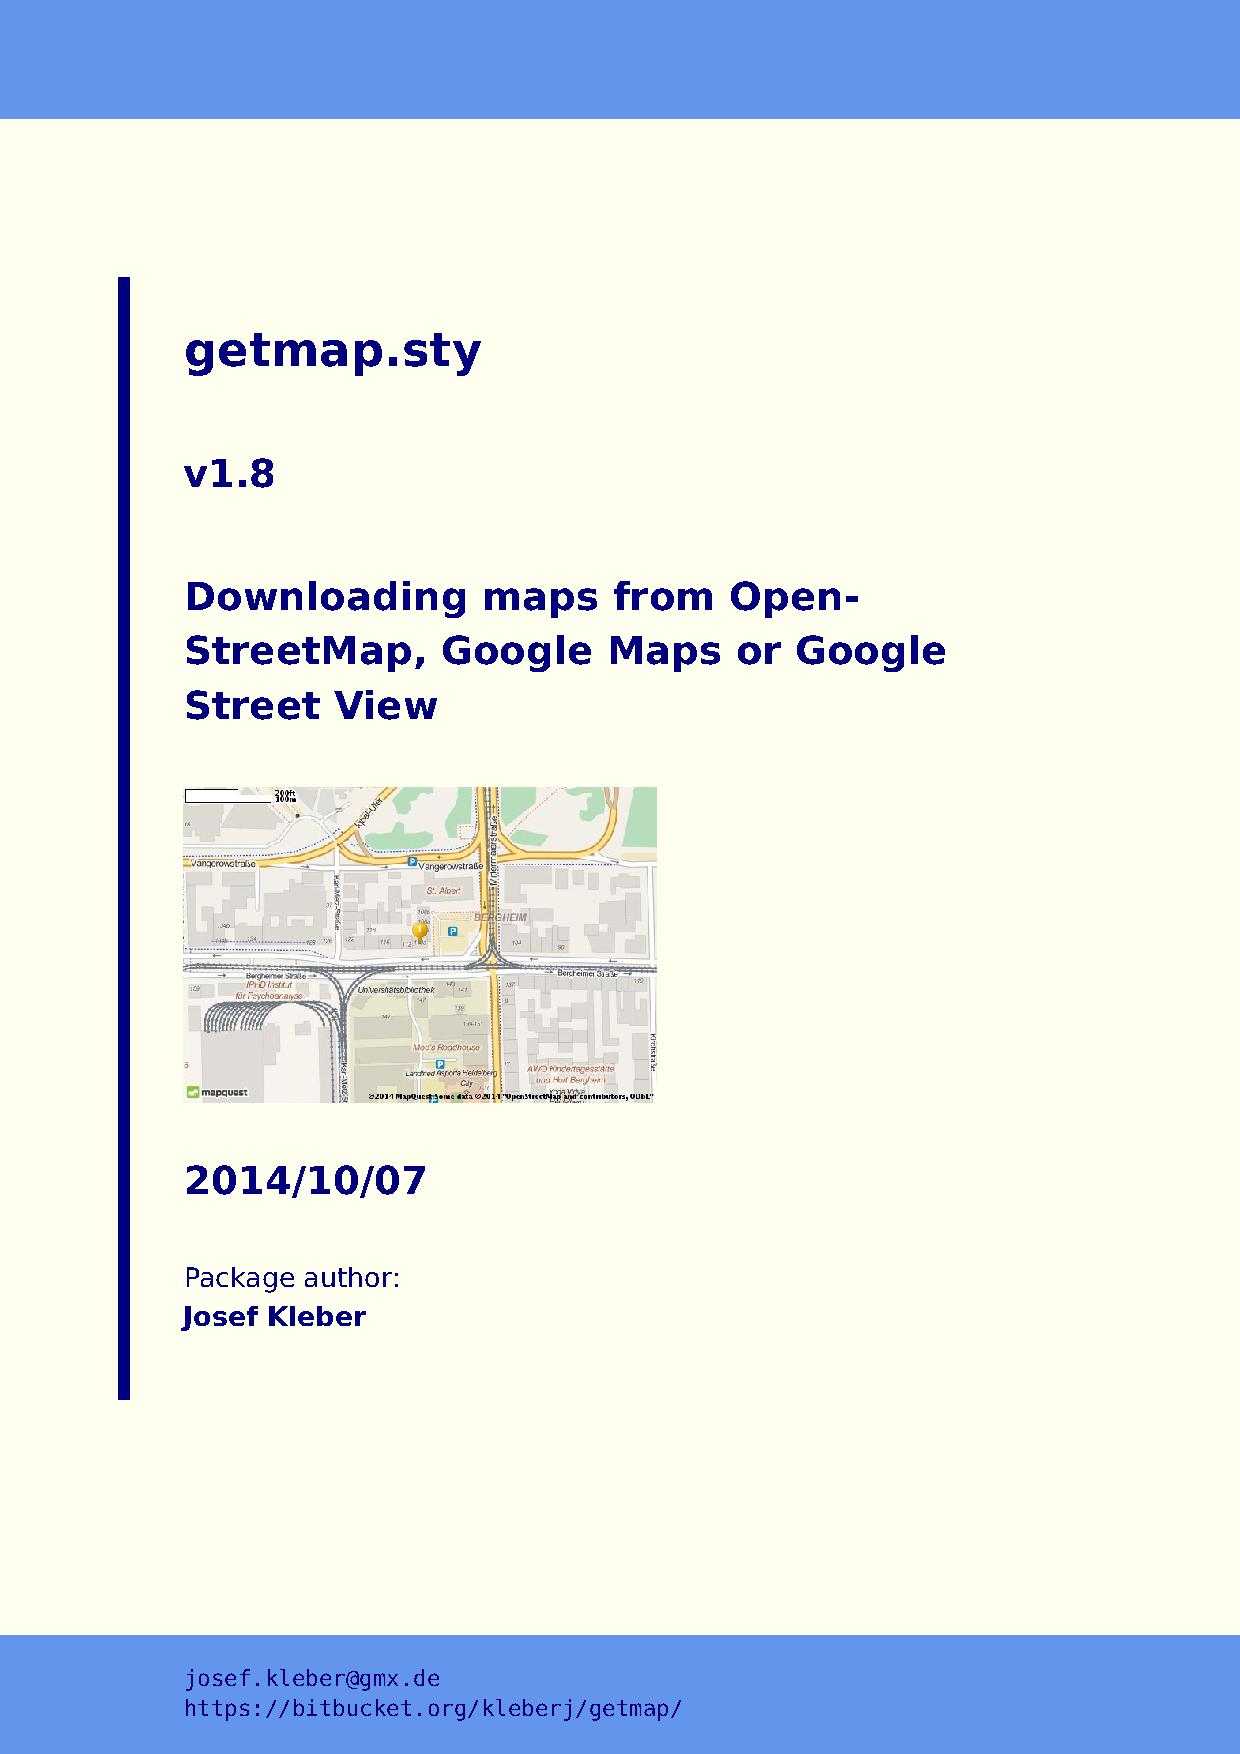
\includegraphics[width=8cm]{getmap}};%
          \draw[anchor=west,yshift=-18cm,xshift=3cm,color=NavyBlue] (0,0) node%
            {\parbox{15cm}{\huge\sffamily\textbf{\@date}}};%
          \draw[anchor=west,yshift=-20cm,xshift=3cm,color=NavyBlue] (0,0) node%
            {\parbox{15cm}{\Large\sffamily{\@authorline\\\textbf{\@author}}}};%
        \end{tikzpicture}%
      };%
      \node[yshift=0cm] at (current page.south west)%
      {%
        \begin{tikzpicture}[remember picture, overlay]%
          \draw[fill=NavyBlue,color=NavyBlue,yshift=6cm,xshift=2cm] (0,0) rectangle (0.2cm,19cm);%
          \draw[fill=CornflowerBlue,color=CornflowerBlue] (0,0) rectangle (\paperwidth,2cm);%
          \draw[anchor=west,yshift=1cm,xshift=3cm,color=NavyBlue] (0,0) node%
            {\parbox{15cm}{\large\sffamily{\@refline}}};%
        \end{tikzpicture}%
      };%
    \end{tikzpicture}%
  \end{titlepage}%
  \pagecolor{white}%
}%
%
\newcommand*{\@tikzhead}[1]%
{%
  \begin{tikzpicture}[remember picture,overlay]%
    \node[yshift=-2cm] at (current page.north west)%
    {%
      \begin{tikzpicture}[remember picture, overlay]%
        \draw[fill=CornflowerBlue] (0,0) rectangle (\paperwidth,2cm);%
        \draw[anchor=west,yshift=1cm,xshift=1.5cm,color=NavyBlue] (0,0) node%
          {\parbox{15cm}{\LARGE\sffamily\textbf{\@title}}};%
        \node[anchor=east,xshift=.9\paperwidth,rectangle,%
              rounded corners=15pt,inner sep=11pt,fill=NavyBlue]%
              {\color{white}\textsc{#1}};%
      \end{tikzpicture}%
    };%
  \end{tikzpicture}%
}%
\clearscrheadings%
\ihead{\@tikzhead{\headmark}}%
\cfoot{\upshape\thepage}%
\pagestyle{scrheadings}%
%
\newcommand*{\Headline}[1]{\@mkboth{#1}{#1}}%
%
\renewcommand{\headfont}{\normalfont\mdseries\scshape}
%
\gdef\@subtitle{}%
\providecommand*{\Subtitle}[1]{\gdef\@subtitle{#1}}%
\gdef\@fileversion{}%
\providecommand*{\Fileversion}[1]{\gdef\@fileversion{#1}}%
\gdef\@author{}%
\providecommand*{\Author}[1]{\gdef\@author{#1}}%
\gdef\@authorline{Package author:}%
\providecommand*{\Authorline}[1]{\gdef\@authorline{#1}}%
\gdef\@refline{}%
\providecommand*{\Refline}[1]{\gdef\@refline{#1}}%
\gdef\and{\unskip{}, }%
\newcommand\doubledash{-\kern0.5pt-}
\def\enoteformat{\rightskip\z@ \leftskip\z@ \parindent=1em\leavevmode\llap{\makeenmark}}
\def\XeLaTeX{Xe\LaTeX}%
%
\newenvironment{optionlist}
{\begin{trivlist}\setlength\leftskip{2em}}
{\end{trivlist}}
\newcommand\optitem[3]{\item [\texttt{\textbf{\textcolor{DodgerBlue}{#1}} \lbrack\textcolor{Crimson}{#2}\rbrack}] #3}
\renewcommand\tableofcontents%
{%
  %\section*{\contentsname}%
  \@mkboth{%
  \MakeUppercase\contentsname}{\MakeUppercase\contentsname}%
  \@starttoc{toc}%
}%
%
\newcommand\env[1]{\texttt{#1}}%
\newcommand\layer[1]{\texttt{#1}\SortIndex{#1}{\texttt{#1} (PGF layer)}%
                     \SortIndex{PGF layer>#1}{\texttt{#1}}}%
\newcommand\styleoption[1]{\texttt{#1}\SortIndex{#1}{\texttt{#1} (Style option)}%
                     \SortIndex{Style option>#1}{\texttt{#1}}}%
\newcommand\envoption[1]{\texttt{#1}\SortIndex{#1}{\texttt{#1} (Puzzle option)}%
                     \SortIndex{Puzzle option>#1}{\texttt{#1}}}%
\newcommand\stylename[1]{\texttt{#1}\SortIndex{#1}{\texttt{#1} (Style file)}%
                     \SortIndex{Style file>#1}{\texttt{#1}}}%
\newcommand\package[1]{\texttt{#1}\SortIndex{#1}{\texttt{#1} (Package)}%
                     \SortIndex{Package>#1}{\texttt{#1}}}%
\newcommand*\margcs[1]{\marginnote{\hbadness=10000\RaggedLeft\scriptsize #1}}%
\def\PrintIndex{\clearpage\Headline{Index}\@input@{\jobname.ind}%
                \global\let\PrintIndex\@empty}
                \renewenvironment{theindex}
               {\if@twocolumn
                  \@restonecolfalse
                \else
                  \@restonecoltrue
                \fi
                \columnseprule \z@
                \columnsep 35\p@
\def\see##1##2{\textit{See} ##1}%
\def\seealso##1##2{\textit{See also} ##1}%
\long\def\cmd##1{\cs{\expandafter\cmd@to@cs\string##1}}%
\def\@url##1{\url@break\ttt{##1}\endgroup}%
\def\ttt{\begingroup\@sanitize\ttfamily\@ttt}%
\def\@ttt##1{##1\endgroup}%
\mathchardef\save@secnumdepth\c@secnumdepth
\c@secnumdepth\m@ne
                \phantomsection%
                \twocolumn%[\section{\indexname}]%
                \refstepcounter{section}
                \addcontentsline{toc}{section}{\protect\numberline{\thesection}Index}%
\c@secnumdepth\save@secnumdepth
                %\thispagestyle{plain}
                \parindent\z@
                \parskip\z@ \@plus .3\p@\relax
                \let\item\@idxitem}
               {\if@restonecol\onecolumn\else\clearpage\fi}
\setlength\parindent{0pt}%
\newcommand*\myref[1]{[see: \ref{#1} on page \pageref{#1}]}
\makeatother
\begin{document}
  \DocInput{\jobname.dtx}
\end{document}
%</driver>
% \fi
%
%\getmap{Bergheimer Straße 110A, 69115 Heidelberg, Germany}
%\GetFileInfo{\jobname.sty}
%\hypersetup{pdfauthor={Josef Kleber},pdftitle={Downloading maps from OpenStreetMap, Google Maps or Google Street View},pdfsubject={Documentation for LaTeX style \filename},pageanchor=true,hyperindex=true}%
%\lstset{language=[LaTeX]TeX,numbers=left,numberstyle=\tiny, basicstyle=\ttfamily, aboveskip=\baselineskip, frame=single, backgroundcolor=\color{LightGoldenrodYellow}, keywordstyle=\color{Blue},
%emph={},emphstyle=\color{Tomato}, 
%emph={[2]width,xsize,ysize,zoom,scale,mode,file,type,heading,pitch,fov,markers,visible,path,pathfile},emphstyle={[2]\color{OliveDrab}},
%morekeywords={getmap,includegraphics}}
%\DoNotIndex{\,,\begingroup,\endgroup,\csname,\def,\else,\endcsname,\equal,\expandafter,
%\fi,\gdef,\ifnum,\ifthenelse,\immediate,\MessageBreak,\NeedsTeXFormat,\newcommand,\newif,
%\PackageInfo,\PackageError,\ProcessOptionsX,\ProvidesPackage,\relax,\RequirePackage,
%\space,\errmessage,\ExecuteOptionsX,}
%
% \bibliographystyle{plain}
% \title{\filename}%
% \Subtitle{Downloading maps from OpenStreetMap, Google Maps or Google Street View}%
% \author{Josef Kleber}
% \Fileversion{\fileversion}
% \date{\filedate}
% \Refline{\href{mailto:josef.kleber@gmx.de}{\texttt{josef.kleber@gmx.de}}\\\href{https://bitbucket.org/kleberj/getmap/}{\texttt{https://bitbucket.org/kleberj/getmap/}}}
% \maketitle
% \stepcounter{page}
% \tableofcontents
% \clearpage
% \setlength\parskip{6pt}%
%
%
%\StopEventually{^^A
% {
% \clearpage
% \raggedright
% \nocite{*}
% \bibliography{getmap}
% }
% \clearpage
%  \PrintChanges
%  \PrintIndex
%}
%
% \Headline{Abstract}
% \begin{abstract}
% The goal of this package is the simplest possible provision of
% map images (OpenStreetMap, Google Maps and Google Street View 
% are supported). In the simplest case, the specification of an
% address is sufficient. The package loads the map using the
% \cmd\write18 feature, which you must activate to use this package.
% The image will be downloaded by an external Lua script. You can 
% use this script also from the command line.
% \end{abstract}
% \vfill
% \renewcommand*{\abstractname}{Acknowledgment}
% \begin{abstract}
% I want to thank Norbert Preining, who did most of the recoding of \texttt{osmimage}
% (\texttt{Bash} $\rightarrow$ \texttt{Lua}). Moreover many thanks to Taco Hoekwater,
% Reinhard Kotucha and Heiko Oberdiek for their valuable contributions.
% Finally, I want to thank Doug Currie for helping me to implement the algorithm
% for encoded polylines in Lua.
% \end{abstract}
% \clearpage
% \section{Options}
% The following options can be used as package options with global scope,
% as well as options for the \cmd\getmap\ command with local scope!
% \subsection{General options}
% \subsubsection[\texttt{mode}]{\texttt{mode (\underline{osm}\textbar{}gm\textbar{}gsv})}
% This option sets the mode, that is the source of the images. OpenStreetMap, Google Maps or Google Street View!
% \subsubsection[\texttt{inputencoding}]{\texttt{inputencoding}}
% This option specifies the input encoding of your file.
% The download script requires the strings encoded in utf8.
% For the safe conversion the input encoding of the file is required.
% Normally, you don't have to specify an encoding.
% The package tries to evaluate the encoding given to \package{inputenc} or assumes utf8.
% Usually that should work.
% \subsubsection[\texttt{overwrite}]{\texttt{overwrite (\underline{false}\textbar{}true)}}
% With this option, you can specify whether the image should be downloaded in any case.
% By default, the option is set to \texttt{false} in order to save bandwidth and compilation time.
% Nevertheless a check is performed on the existence of the image and the
% image will be downloaded, if it is not present.
% In the case of \texttt{true}, the image will be downloaded anyway!
% BTW, \texttt{overwrite} is equivalent to \texttt{overwrite=true}.
% \subsubsection[\texttt{file}]{\texttt{file (\underline{getmap})}}
% This \marginpar{\footnotesize\fbox{\parbox{3cm}{\raggedright{}changed default value to \texttt{getmap} in version 1.2!}}}
% option allows you to specify the name of the image (without extension).
% \subsection{\texttt{osm} mode}
% \subsubsection[\texttt{key}]{\texttt{key (\underline{Fmjtd\textbar{}luur20u22d,75=o5-9aylh6}})}
% In \texttt{osm} mode, the download script requires a key in order to use the service of MapQuest.
% By default, it uses a key, which is registered for \package{getmap}.
% But you can register and use your own key with this option.
% The default key is stored in \texttt{getmap.cfg}. You can copy this file to your local \TeX\ tree
% and store your own key there\footnote{Mapquest will deliver an url-encoded key, which must
% be decoded to ASCII, e.g. by \href{http://urldecode.org/}{Url decode}}!
% This file will be found after running \texttt{texhash}!
% \subsubsection[\texttt{scale}]{\texttt{scale (\underline{3385}})}
% This option allows you to specify a display scale for the map image in the range of
% 1692 -- 221871572. You will not necessarily see a difference between 5000 and 5500.
% A scale value of 3385 corresponds to a zoom level of 17.
% \subsubsection[\texttt{zoom}]{\texttt{zoom}}
% This option allows you to specify a zoom level in the range of 1 -- 18.
% This option overwrites a possibly given scale.
% \subsubsection[\texttt{xsize}]{\texttt{xsize (\underline{600})}}
% This option specifies the width of the map in pixels.
% If \marginpar{\footnotesize\fbox{\parbox{3cm}{\raggedright{}changed default value to \texttt{600} in version 1.2!}}}
% you only want to slightly increase or decrease the map extract,
% you should adjust the size of the map. You still have full control over the size of
% the map in the document with the options of \cmd\includegraphics. (max: 3840)
% \subsubsection[\texttt{ysize}]{\texttt{ysize (\underline{400})}}
% This option specifies the height of the map in pixels. (max: 3840)
% \subsubsection[\texttt{imagetype}]{\texttt{imagetype (\underline{png}\textbar{}jpeg\textbar{}jpg\textbar{}gif)}}
% This option allows you to specify the type of the image.
% \subsubsection[\texttt{type}]{\texttt{type (\underline{map}\textbar{}sat\textbar{}hyb)}}
% This option specifies the type of the map.
% It seems as if there would be only a few regions of Mother Earth,
% for which satellite and hybrid images are available.
% \subsubsection[\texttt{color}]{\texttt{color (\underline{yellow\_1})}}
% This option specifies the color of the marker. Possible colors:
%
% \href{http://open.mapquestapi.com/staticmap/icons.html}{http://open.mapquestapi.com/staticmap/icons.html}
% \subsubsection[\texttt{number}]{\texttt{number (\underline{1})}}
% This option specifies the number of the marker.
% \subsection{\texttt{gm} mode}
% \subsubsection[\texttt{scale}]{\texttt{scale (\underline{1})}}
% For the free version of Google Maps the image size is limited to 640x640.
% You can set \texttt{scale} to a value of 2, to get exactly the same map in doubled size in pixels.
% \subsubsection[\texttt{zoom}]{\texttt{zoom} (\underline{17})}
% This option allows you to specify a zoom level in the range of 0 -- 21.
% \subsubsection[\texttt{xsize}]{\texttt{xsize (\underline{600})}}
% This option specifies the width of the map in pixels.
% If you only want to slightly increase or decrease the map extract,
% you should adjust the size of the map. You still have full control over the size of
% the map in the document with the options of \cmd\includegraphics. (max: 640)
% \subsubsection[\texttt{ysize}]{\texttt{ysize (\underline{400})}}
% This option specifies the height of the map in pixels. (max: 640)
% \subsubsection[\texttt{imagetype}]{\texttt{imagetype (\underline{png}\textbar{}png8\textbar{}
% png32\textbar{}gif\textbar{}jpg} (progressive)\texttt{\textbar{}jpg-baseline} (flat))}
% This option allows you to specify the type of the image.
% \subsubsection[\texttt{type}]{\texttt{type (\underline{roadmap}\textbar{}satellite\textbar{}hybrid\textbar{}terrain)}}
% This option specifies the type of the map.
% \subsubsection[\texttt{color}]{\texttt{color (\underline{blue})}}
% This option specifies the color of the marker. Possible colors:
%
% black, brown, green, purple, yellow, blue, gray, orange, red, white or in hex format \texttt{0x3399FF}
% \subsubsection[\texttt{number}]{\texttt{number (\underline{1})}}
% This option specifies the number of the marker. Google Maps also allows uppercase letters: [A-Z]!
% \subsubsection[\texttt{language}]{\texttt{language} (\underline{en})}
% This option specifies the language of the map labels.
% Of course, not all languages are supported for all countries.
% At least, english and one of the national languages should be supported.
% Possible option values: en, de, fr, es, it, fi, ...
% \subsubsection{\texttt{markers}}
% This option allows you to set more than just the standard marker, which will no longer be used!
% You don't have to specify an address, as Google Maps will deliver an image with all markers on the map.
% Nevertheless, you can specify an address, which will define the center of the map.
% This option expects one or more URL parameters like:
%
% \texttt{\&markers=size:mid\textbar{}color:blue\textbar{}label:S\textbar{}loc1\textbar{}loc2\textbar{}...}
%
% \getmap[file=bmus1, mode=gm,
%         markers={&markers=size:mid|label:B|color:green|Bode Museum, Berlin%
%                  &markers=label:P|color:green|Pergamonmuseum, Berlin%
%                  &markers=label:N|color:blue|Neues Museum, Berlin}%
% ]{}
% \begin{center}\includegraphics[width=10cm]{bmus1}\end{center}
% \iffalse
%<*example>
% \fi
\begin{lstlisting}
\getmap[
file=bmus1, mode=gm,
markers={&markers=size:mid|label:B|color:green|Bode Museum, Berlin%
         &markers=label:P|color:green|Pergamonmuseum, Berlin%
         &markers=label:N|color:blue|Neues Museum, Berlin}%
]{}
\includegraphics[width=10cm]{bmus1}
\end{lstlisting}
% \iffalse
%</example>
% \fi
% The parameters size, color and label are optional!
% \begin{description}
% \item[size] tiny, \underline{mid}, small
% \item[color] \underline{red}, black, brown, green, purple, yellow, blue, gray, orange, white, 0x1188FF
% \item[label] [0-9][A-Z] (only in mid size!)
% \end{description}
% The default is a mid-sized red bubble with a black point!
% \subsubsection{\texttt{visible}}
% With this option you can specify a list of locations (separated by a pipe), which must be on the map!
%
% \getmap[file=bmus2, mode=gm,
%        markers={&markers=size:mid|label:B|color:green|Bode Museum, Berlin
%                 &markers=label:P|color:green|Pergamonmuseum, Berlin
%                 &markers=label:N|color:blue|Neues Museum, Berlin},
%        visible={Brandenburger Tor, Berlin|Reichstagsufer 1, Berlin}]{}
% \begin{center}\includegraphics[width=10cm]{bmus2}\end{center}
% \iffalse
%<*example>
% \fi
\begin{lstlisting}
\getmap[
file=bmus2, mode=gm
markers={&markers=size:mid|label:B|color:green|Bode Museum, Berlin%
         &markers=label:P|color:green|Pergamonmuseum, Berlin%
         &markers=label:N|color:blue|Neues Museum, Berlin},%
visible={Brandenburger Tor, Berlin|Reichstagsufer 1, Berlin}]{}
\includegraphics[width=10cm]{bmus2}
\end{lstlisting}
% \iffalse
%</example>
% \fi
% \subsubsection{\texttt{path}}
% With this option you can define one or more paths! It expects one or more URL parameters like:
%
% \texttt{\&path=weight:5\textbar{}color:orange\textbar{}loc1\textbar{}loc2\textbar{}...}
%
% \iffalse
%<*example>
% \fi
\begin{lstlisting}
\getmap[file=bmus3, mode=gm, language=de,
markers={&markers=size:mid|label:B|color:green|Bode Museum, Berlin%
         &markers=label:P|color:green|Pergamonmuseum, Berlin%
         &markers=label:N|color:blue|Neues Museum, Berlin},%
path={&path=weight:5|color:orange|Bode Museum, Berlin|%
      Pergamonmuseum, Berlin|Neues Museum, Berlin|%
      James-Simon-Park,Berlin|52.522649,13.402523%
      &path=weight:5|color:purple|James-Simon-Park, Berlin|%
      Weinmeisterstraße 6, Berlin}]{}
\includegraphics[width=10cm]{bmus3}
\end{lstlisting}
% \iffalse
%</example>
% \fi
%
% \getmap[file=bmus3, mode=gm, language=de,
%        markers={&markers=size:mid|label:B|color:green|Bode Museum, Berlin%
%                 &markers=label:P|color:green|Pergamonmuseum, Berlin%
%                 &markers=label:N|color:blue|Neues Museum, Berlin},%
%        path={&path=weight:5|color:orange|Bode Museum, Berlin|%
%              Pergamonmuseum, Berlin|Neues Museum, Berlin|%
%              James-Simon-Park,Berlin|52.522649,13.402523%
%              &path=weight:5|color:purple|James-Simon-Park, Berlin|%
%              Weinmeisterstraße 6, Berlin}]{}
% \begin{center}\includegraphics[width=10cm]{bmus3}\end{center}
%
% You can also use \texttt{fillcolor} to mark areas! In paths, you
% can also specify RGB32 colors, in which the last byte defines opacity,
% e.g. 55 (33\%).
%
% \getmap[file=cpny, mode=gm, zoom=13,
%        path={&path=weight:2|color:orange|fillcolor:0xff641A55|
%              40.764302, -73.973004|40.768044, -73.981903|%
%              40.800642, -73.958193|40.796887, -73.949226|%
%              40.764302, -73.973004}]{Central Park, New York}
% \begin{center}\includegraphics[width=10cm]{cpny}\end{center}
% \iffalse
%<*example>
% \fi
\begin{lstlisting}
\getmap[file=cpny, mode=gm, zoom=13,
       path={&path=weight:2|color:orange|fillcolor:0xff641A55|
             40.764302, -73.973004|40.768044, -73.981903|%
             40.800642, -73.958193|40.796887, -73.949226|%
             40.764302, -73.973004}]{Central Park, New York}
\includegraphics[width=10cm]{cpny}
\end{lstlisting}
% \iffalse
%</example>
% \fi
%
% With small enough spaces between way points you can also defines routes!
% \subsubsection{\texttt{pathfile}}
% This option specifies the file holding the path specification. It will be loaded by the \texttt{Lua} script.
% You can use the \env{filecontents*} environment to keep the definition in your document.
% It should be a one line utf8-encoded file!
% \subsection{\texttt{gsv} mode}
% \subsubsection[\texttt{xsize}]{\texttt{xsize (\underline{600})}}
% This option specifies the width of the map in pixels. (max: 640)
% \subsubsection[\texttt{ysize}]{\texttt{ysize (\underline{400})}}
% This option specifies the height of the map in pixels. (max: 640)
% \subsubsection[\texttt{heading}]{\texttt{heading (\underline{0})}}
% This option specifies the heading (direction) in degrees in the range of 0 -- 360. (0: north, 90: east, ...)
% \subsubsection[\texttt{pitch}]{\texttt{pitch (\underline{0})}}
% This option specifies the pitch (angle) of the camera view in degrees in the range of -90 -- 90.
% \subsubsection[\texttt{fov}]{\texttt{fov (\underline{90})}}
% This option specifies the field of horizontal view (kind of zoom) in degrees in the range of 0 -- 120.
% \section{Command(s)}
% \subsection[\textbackslash{}getmap]{\cmd\getmap}
% With the \cmd\getmap\ command\margcs{\cmd\getmap\oarg{options}\marg{address}} you can download
% a map, if you enable \cmd\write18 (TeXLive: \texttt{-shell-escape}, MiKTeX: \texttt{-{}-enable-write18}).
% This is only necessary if you actually download an image.
% You can use the options described above to specify the properties of the downloaded image.
% After executing the command, the image is available in the current working directory!
%
% In the simplest case, you only need an address, a POI or geographic coordinates
% (\texttt{latitude,longitude}) to download the map. \marg{address} must be fully expanded and must not contain macros!
% By default, the image is saved under the name \texttt{getmap.png}!
% If you need only one map (e.g. the office of Dante e.V.) in your document, it can be as simple as:
%
% \begin{center}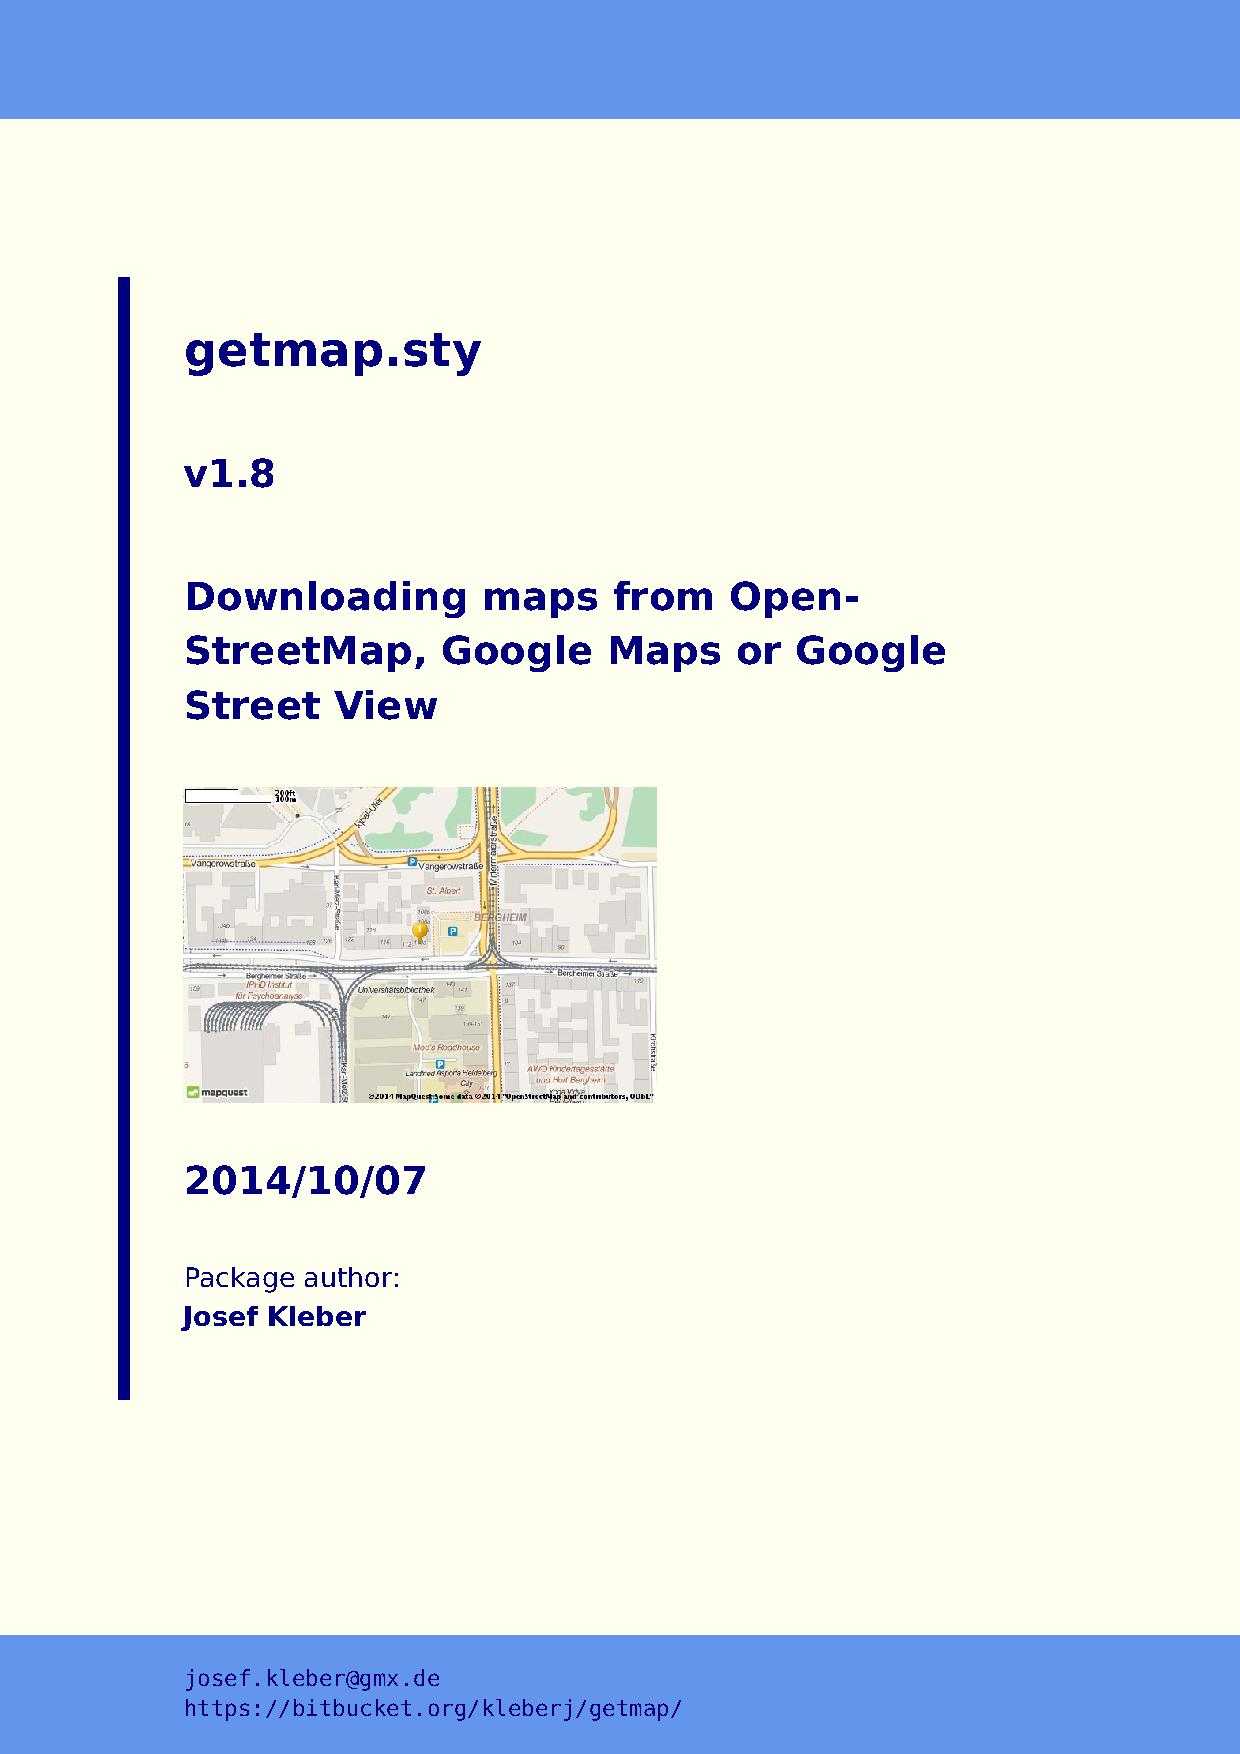
\includegraphics[width=9cm]{getmap}\end{center}
%
% \iffalse
%<*example>
% \fi
\begin{lstlisting}
\getmap{Bergheimer Straße 110A, 69115 Heidelberg, Germany}
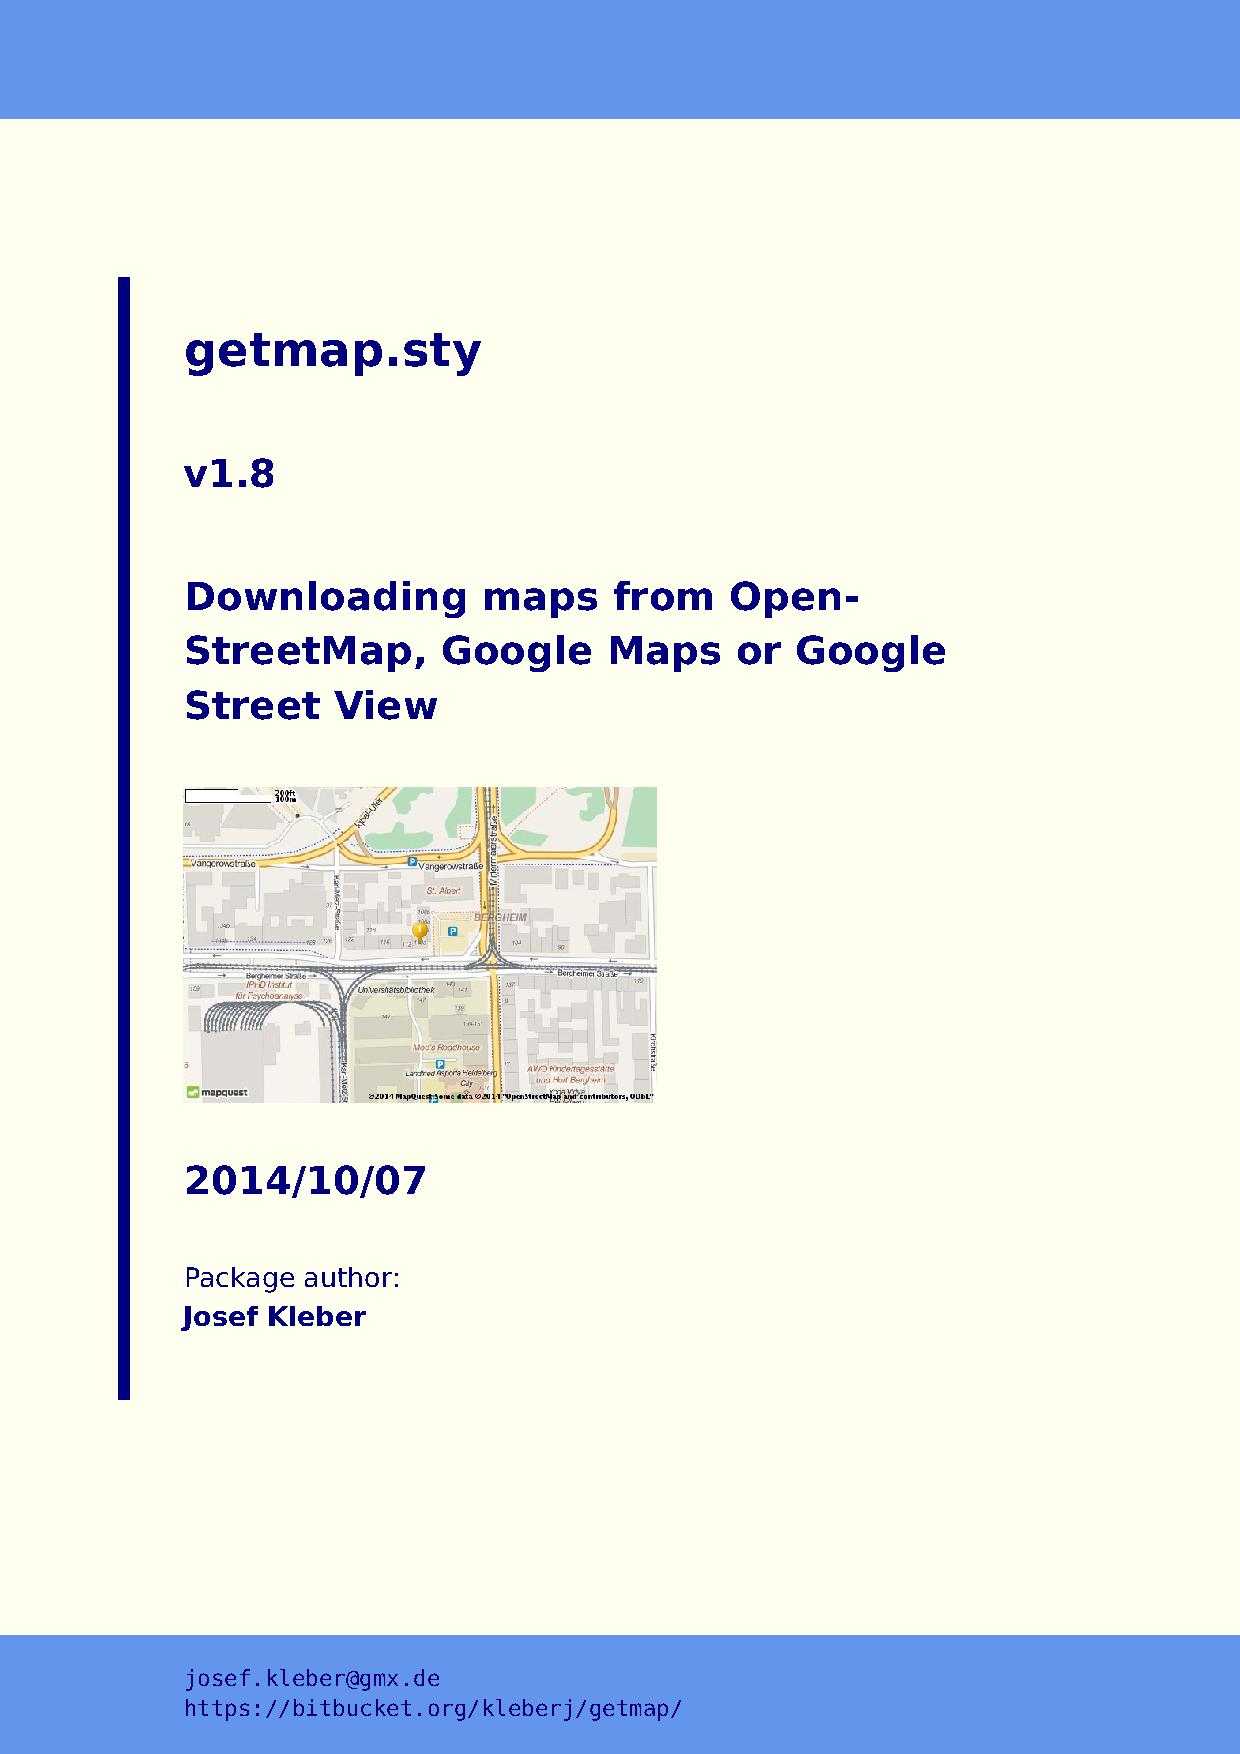
\includegraphics[width=9cm]{getmap}
\end{lstlisting}
% \iffalse
%</example>
% \fi
%
% \clearpage
% \section{Examples}\marginnote{\attachfile[author={Josef Kleber},subject={getmap-example.tex},description={getmap-example.tex (source example)} ,mimetype={text/plain}, icon={Tag}]{getmap-example.tex}}
%
% The same map as before from Google Maps:
%
% \getmap[file=dantegm,mode=gm]{Bergheimer Straße 110A, 69115 Heidelberg, Germany}
% \begin{center}\includegraphics[width=9cm]{dantegm}\end{center}
% \iffalse
%<*example>
% \fi
\begin{lstlisting}
\getmap[file=dantegm,mode=gm]{Bergheimer Straße 110A,%
                              69115 Heidelberg, Germany}
\includegraphics[width=9cm]{dantegm}
\end{lstlisting}
% \iffalse
%</example>
% \fi
%
% The same map as satellite image:
%
% \getmap[file=dantegmsat,mode=gm,type=satellite]{Bergheimer Straße 110A, 69115 Heidelberg, Germany}
% \begin{center}\includegraphics[width=9cm]{dantegmsat}\end{center}
% \iffalse
%<*example>
% \fi
\begin{lstlisting}
\getmap[file=dantegmsat,mode=gm,type=satellite]
       {Bergheimer Straße 110A, 69115 Heidelberg, Germany}
\includegraphics[width=9cm]{dantegmsat}
\end{lstlisting}
% \iffalse
%</example>
% \fi
% \clearpage
% L'afrique, mon amour!
% 
% \getmap[file=africa,mode=gm,type=terrain,xsize=500,ysize=500,scale=2,zoom=3]{0,16}
% \begin{center}\includegraphics[width=9cm]{africa}\end{center}
% \iffalse
%<*example>
% \fi
\begin{lstlisting}
\getmap[file=africa,mode=gm,type=terrain,xsize=500,ysize=500,%
        scale=2,zoom=3]{0,16}
\includegraphics[width=9cm]{africa}
\end{lstlisting}
% \iffalse
%</example>
% \fi
% L'amour, ...
% 
% \getmap[file=paris,mode=gm,type=hybrid,xsize=500,ysize=300,scale=2,zoom=16]{Tour Eiffel, Paris}
% \begin{center}\includegraphics[width=9cm]{paris}\end{center}
% \iffalse
%<*example>
% \fi
\begin{lstlisting}
\getmap[file=paris,mode=gm,type=hybrid,xsize=500,ysize=300,%
        scale=2,zoom=16]{Tour Eiffel, Paris}
\includegraphics[width=9cm]{paris}
\end{lstlisting}
% \iffalse
%</example>
% \fi
% \clearpage
% Street View now:
% 
% \getmap[file=parisgsv,mode=gsv,heading=320,pitch=30,fov=40,xsize=300,ysize=600]{Avenue Piere-Loti, Paris}
% \begin{center}\includegraphics[width=4cm]{parisgsv}\end{center}
% \iffalse
%<*example>
% \fi
\begin{lstlisting}
  \getmap[file=parisgsv,mode=gsv,heading=320,pitch=30,fov=40,%
          xsize=300,ysize=600]{Avenue Piere-Loti, Paris}
  \includegraphics[width=4cm]{parisgsv}
\end{lstlisting}
% \iffalse
%</example>
% \fi
%
% and from the platform:
% 
% \getmap[file=parisgsvp,mode=gsv,heading=30,pitch=-25,fov=60]{Tour Eiffel, Paris}
% \begin{center}\includegraphics[width=8cm]{parisgsvp}\end{center}
% \iffalse
%<*example>
% \fi
\begin{lstlisting}
  \getmap[file=parisgsvp,mode=gsv,heading=30,pitch=-25,fov=60]%
         {Tour Eiffel, Paris}
  \includegraphics[width=8cm]{parisgsvp}
\end{lstlisting}
% \iffalse
%</example>
% \fi
% \section{The \texttt{getmapdl} Lua script}
% Basically, the \texttt{getmapdl} Lua script downloads static map images
% depending on command line options and allows to parse \texttt{kml}, \texttt{gpx} and
% \texttt{gps} (a plain list of geographical coordinate pairs \texttt{(latitude,longitude)}
% on each line) files and outputs \texttt{gps} or encoded polylines (epl).
% The script offers the following modes (\texttt{-m}):
% \begin{description}
% \item[osm] downloads a static map image based on OpenStreetMap data
% \item[gm] downloads a static map image based on Google Maps data
% \item[gsv] downloads an image based on Google Street View data
% \item[kml2epl] parses a \texttt{kml} file and outputs geographical coordinates of places and
% encoded polylines (\texttt{epl}) for routes and lines  to \texttt{STDOUT}
% \item[kml2gps] parses a \texttt{kml} file and outputs geographical coordinates
% \item[gpx2epl] parses a \texttt{gpx} file and outputs encoded polylines 
% \item[gpx2gps] parses a \texttt{gpx} file and outputs a list of geographic coordinate pairs (\texttt{gps})
% \item[gps2epl] parses a \texttt{gps} file and outputs \texttt{epl}
% \item[gps2gps] parses a \texttt{gps} file and outputs -- based on a given bound -- a reduced list of \texttt{gps} coordinates
% \end{description}
% The first three modes are used by \cmd\getmap. You may use the script also from the command line!
% \texttt{getmapdl -h} will give you a list of available commad line options.
%
% The other modes are usefull for creating encoded polylines (\texttt{epl}), which is
% the route format of Google Maps. You can parse the following example from Google Maps in \texttt{gpx} format
% \iffalse
%<*example>
% \fi
\begin{lstlisting}
<trkseg>
      <trkpt lon="-120.2" lat="38.5"/>
      <trkpt lon="-120.95" lat="40.7"/>
      <trkpt lon="-126.453" lat="43.252"/>
</trkseg>
\end{lstlisting}
% \iffalse
%</example>
% \fi
% with
% \iffalse
%<*example>
% \fi
\begin{lstlisting}
$ getmapdl -m gpx2epl -G test.gpx
_p~iF~ps|U_ulLnnqClqNvxq`@

\end{lstlisting}
% \iffalse
%</example>
% \fi
% This encoded polyline can be used for the \texttt{path} or \texttt{pathfile}
% option of \cmd\getmap.
% \section{How to define routes}
% Routes are described by so called encoded polylines and can be used with
% \texttt{enc:polyline\_data} as location specifier in a \texttt{path}.
% This string can contain all sorts of troublesome characters for \LaTeX{}.
% \cmd\getmap\ can deal with them, with the exception of curly braces!
% These will break your \LaTeX{} document. As a work-around, use the \texttt{pathfile} option.
% Please note that the length of the URL is limited to 2048 bytes. So, there's
% no way to support extreme long paths!
% \subsection{OpenStreetMap}
% OpenStreetMap does not offer routing service directly, but you can
% use an OpenStreetMap based route service\footnote{\href{http://openrouteservice.org}{http://openrouteservice.org}}
% to create your route and export it to a \texttt{gpx} file\footnote{This also means that you can visualize your own routes tracked with hardware or a software app!}.
% It's basically a xml-packaged list of geographical coordinates.
% You can use the \texttt{getmapdl} script to convert a route to encoded polylines, e.g.
% a pedestrian route from Berlin Central Station to Brandenburg Gate:
%
% \begin{filecontents*}{berlin.epl}
% &path=weight:5|color:purple|enc:_xq_IcgrpA?AFE@?^BFE@A^U@CLQXEZU?gCR?B?DBF@@?vA?D?D?BAHE@JBN@JLGFCG[DC~C?@?F?R?vA?p@iB@i@Fe@JWRSTOf@Gh@C^A?e@?gE?w@r@?lB@hA?`@??M?aA?]dI??O?O?Cn@cBfBeF|AeEHNVNBc@H@H_AEwA?OAMNA@N
% \end{filecontents*}
% \getmap[file=berlin, mode=gm, language=de, scale=2,
%         xsize=400, ysize=600,
%         markers={&markers=size:mid|label:H|color:green|Berlin, Hbf
%                  &markers=label:B|color:blue|Brandenburger Tor, Berlin},
%         pathfile={berlin.epl}]{}
% \begin{center}\includegraphics[width=6cm]{berlin}\end{center}
%
% \iffalse
%<*example>
% \fi
\begin{lstlisting}
\begin{filecontents*}{berlin.epl}
&path=weight:5|color:purple|enc:_xq_IcgrpA?AFE@?^BFE@A^U@CLQXEZU?
gCR?B?DBF@@?vA?D?D?BAHE@JBN@JLGFCG[DC~C?@?F?R?vA?p@iB@i@Fe@JWRSTO
f@Gh@C^A?e@?gE?w@r@?lB@hA?`@??M?aA?]dI??O?O?Cn@cBfBeF|AeEHNVNBc@H
@H_AEwA?OAMNA@N
\end{filecontents*}
\getmap[file=berlin, mode=gm, language=de, scale=2,
        xsize=400, ysize=600,
markers={&markers=size:mid|label:H|color:green|Berlin, Hbf
         &markers=label:B|color:blue|Brandenburger Tor, Berlin},
pathfile={berlin.epl}]{}
\includegraphics[width=6cm]{berlin}
\end{lstlisting}
% \iffalse
%</example>
% \fi
%
% \subsection{Google Maps}
% One possible way is to use Google Maps'
% online interactive map tool\footnote{\href{https://developers.google.com/maps/documentation/utilities/polylineutility}{https://developers.google.com/maps/documentation/utilities/polylineutility}}!
%
% \begin{filecontents*}{muc.epl}
% &path=weight:5|color:orange|enc:okydHa}peAXOHi@jANv@A@kJJmFAiDJuAHmDXcBb@cC`@gC^_DV}CJaCF{APaBVkBdAyEf@qC`@{B\aDSwB
% \end{filecontents*}
% \getmap[file=muc, mode=gm,
%         markers={&markers=size:mid|label:H|color:green|München, Hbf
%                  &markers=label:S|color:yellow|Stachus, München
%                  &markers=label:M|color:blue|Marienplatz, München},
%         pathfile={muc.epl}]{}
% \begin{center}\includegraphics[width=10cm]{muc}\end{center}
%
% \iffalse
%<*example>
% \fi
\begin{lstlisting}
\begin{filecontents*}{muc.epl}
&path=weight:5|color:orange|enc:okydHa}peAXOHi@jANv@A@kJJmFAiDJuA
HmDXcBb@cC`@gC^_DV}CJaCF{APaBVkBdAyEf@qC`@{B\aDSwB
\end{filecontents*}
\getmap[file=muc, mode=gm,
markers={&markers=size:mid|label:H|color:green|München, Hbf
         &markers=label:S|color:yellow|Stachus, München
         &markers=label:M|color:blue|Marienplatz, München},
pathfile={muc.epl}]{}
\includegraphics[width=10cm]{muc}
\end{lstlisting}
% \iffalse
%</example>
% \fi
%
% You can also use the \textbf{new} version of \textit{My Maps}.
% It allows you to define markers, routes and arbitrary lines on
% different layers and to export these into a \texttt{kml} file,
% e.g \href{https://bitbucket.org/kleberj/getmap/downloads/Berlin.kml}{berlin.kml}\footnote{\href{https://bitbucket.org/kleberj/getmap/downloads/Berlin.kml}{https://bitbucket.org/kleberj/getmap/downloads/Berlin.kml}}:
%
% \iffalse
%<*example>
% \fi
\begin{lstlisting}
$ getmapdl -m kml2epl -K Berlin.kml
Route: Route von Berlin Hbf, Moabit nach Brandenburger Tor, Paris
er Platz, Berlin
k}q_IufrpA?iFQ?gCDQBMHSm@Wq@GQIK]{AUaA}AaICIMm@Kg@EUiByIi@cDSqA_@
uBIa@a@gBpB[fAMhCS|@Gd@Ev@Ep@GfAIpC[bAMr@IbAMp@G\GtBUdCSp@MrAK~AQ
pAMhAKx@IjDc@VAB?D@@?B?dCU`AKjAMRCPlGNtEBhABh@BVF`@D`@D\rB{@ZKDAH
CLAHAHBHBFHFFDNHRHJHHDDHDHBF?F?VCJCJILQJUJg@HQJMJKHAFAJ?X?bCRH@R?
AWQ?K@iBKq@GYAK@EBIFEFEFEFCFAD


Point: Berlin Hbf, Moabit  [Europaplatz 1, 10557 Berlin, Deutschl
and]
52.52581820000001,13.3695451


Point: Brandenburger Tor, Pariser Platz, Berlin  [Ebertstraße 21,
 10117 Berlin, Deutschland]
52.5159099,13.3773202


Point: Berlin Hbf  [arrive with train]
52.5249948,13.368988


Point: Reichstag  [nice view from the roof]
52.5185973,13.3758974


Point: Brandenburger Tor  [once behind the wall]
52.5163514,13.3789873


Route: Route von Berlin Hbf, Moabit nach Pariser Platz, Berlin
k}q_IufrpA?iFQ?@hH@H@F@B@B@?DB?\?|B@F@DB@B@~FCB?X@V??O?O?O?wF@W?o
@?k@?Y?eAvAD`@?`@ARCFAP?hAAZ?B?D?J?B?DAJB^@T?~B?MsAAIAEAM?S@OBM?A
@IDKBKDKFKFIJEFCJAJATAL?XAN?P?VAlBCbB?L@RB?kH@}Gp@]|@ObA?BAz@JTF^
LZN?wF@aCE]~Am@\KREJCNANAH@HBJHHFLPP\DBFFDB@@@?D@F?JAJCKiEAQ?K@I?
KBSXC


Point: Berlin Hbf, Moabit  [Europaplatz 1, 10557 Berlin, Deutschl
and]
52.52581820000001,13.3695451


Point: Deutscher Bundestag Redaktion Das Parlament, Berlin  [Plat
z der Republik 1, 10557 Berlin, Deutschland]
52.518502000000005,13.3751849


Point: Pariser Platz, Berlin  [Pariser Platz 1, 10117 Berlin, Deu
tschland]
52.5160749,13.3783013

\end{lstlisting}
% \iffalse
%</example>
% \fi
%
% Now, you can take these data for your map:
%
% \begin{filecontents*}{berlin2.epl}
% &path=weight:5|color:orange|enc:k}q_IufrpA?iFQ?@hH@H@F@B@B@?DB?\?|B@F@DB@B@~FCB?X@V??O?O?O?wF@W?o@?k@?Y?eAvAD`@?`@ARCFAP?hAAZ?B?D?J?B?DAJB^@T?~B?MsAAIAEAM?S@OBM?A@IDKBKDKFKFIJEFCJAJATAL?XAN?P?VAlBCbB?L@RB?kH@}Gp@]|@ObA?BAz@JTF^LZN?wF@aCE]~Am@\KREJCNANAH@HBJHHFLPP\DBFFDB@@@?D@F?JAJCKiEAQ?K@I?KBSXC&path=weight:5|color:purple|enc:k}q_IufrpA?iFQ?gCDQBMHSm@Wq@GQIK]{AUaA}AaICIMm@Kg@EUiByIi@cDSqA_@uBIa@a@gBpB[fAMhCS|@Gd@Ev@Ep@GfAIpC[bAMr@IbAMp@G\GtBUdCSp@MrAK~AQpAMhAKx@IjDc@VAB?D@@?B?dCU`AKjAMRCPlGNtEBhABh@BVF`@D`@D\rB{@ZKDAHCLAHAHBHBFHFFDNHRHJHHDDHDHBF?F?VCJCJILQJUJg@HQJMJKHAFAJ?X?bCRH@R?AWQ?K@iBKq@GYAK@EBIFEFEFEFCFAD
% \end{filecontents*}
% \getmap[file=berlin2, language=de, xsize=400, ysize=600, scale=2, mode=gm,
%         markers={&markers=size:mid|label:H|color:green|52.5249948,13.368988
%                  &markers=size:mid|label:R|color:yellow|52.5185973,13.3758974
%                  &markers=label:B|color:blue|52.5163514,13.3789873},
%         pathfile={berlin2.epl}]{}
% \begin{center}\includegraphics[width=6cm]{berlin2}\end{center}
%
% \iffalse
%<*example>
% \fi
\begin{lstlisting}
\begin{filecontents*}{berlin2.epl}
&path=weight:5|color:orange|enc:k}q_IufrpA?iFQ?@hH@H@F@B@B@?DB?\?
|B@F@DB@B@~FCB?X@V??O?O?O?wF@W?o@?k@?Y?eAvAD`@?`@ARCFAP?hAAZ?B?D?
J?B?DAJB^@T?~B?MsAAIAEAM?S@OBM?A@IDKBKDKFKFIJEFCJAJATAL?XAN?P?VAl
BCbB?L@RB?kH@}Gp@]|@ObA?BAz@JTF^LZN?wF@aCE]~Am@\KREJCNANAH@HBJHHF
LPP\DBFFDB@@@?D@F?JAJCKiEAQ?K@I?KBSXC&path=weight:5|color:purple|
enc:k}q_IufrpA?iFQ?gCDQBMHSm@Wq@GQIK]{AUaA}AaICIMm@Kg@EUiByIi@cDS
qA_@uBIa@a@gBpB[fAMhCS|@Gd@Ev@Ep@GfAIpC[bAMr@IbAMp@G\GtBUdCSp@MrA
K~AQpAMhAKx@IjDc@VAB?D@@?B?dCU`AKjAMRCPlGNtEBhABh@BVF`@D`@D\rB{@Z
KDAHCLAHAHBHBFHFFDNHRHJHHDDHDHBF?F?VCJCJILQJUJg@HQJMJKHAFAJ?X?bCR
H@R?AWQ?K@iBKq@GYAK@EBIFEFEFEFCFAD
\end{filecontents*}
\getmap[file=berlin2, language=de, xsize=400, ysize=600,
        scale=2, mode=gm,
markers={&markers=size:mid|label:H|color:green|52.5249948,13.3689
88
         &markers=size:mid|label:R|color:yellow|52.5185973,13.375
8974
         &markers=label:B|color:blue|52.5163514,13.3789873},
pathfile={berlin2.epl}]{}%
\includegraphics[width=6cm]{berlin2}%
\end{lstlisting}
% \iffalse
%</example>
% \fi
%
% \subsubsection{Long routes}
%
% Long routes are defined by a huge number of way points, but the URL length
% is limited to 2048 bytes. The following \href{https://bitbucket.org/kleberj/getmap/downloads/MucBer.kml}{example}\footnote{https://bitbucket.org/kleberj/getmap/downloads/MucBer.kml}
% (Stachus, Munich $\rightarrow$ Brandenburg Gate, Berlin) consists of more
% than 6000 way points. A created polyline would hugely exceed the URL length limit!
%
% After transfering the \texttt{kml} file into a \texttt{gps} file, you can use
% the \texttt{gps2gps} mode of \texttt{getmapdl} to reduce the number of
% way points by a given bound. It takes a new pair of \texttt{gps} coordinates
% only if the difference of latitude or longitude is larger than the given bound!
% Finally, you can use the new \texttt{gps} file to create an encoded polyline.
%
% \iffalse
%<*example>
% \fi
\begin{filecontents*}{mucber.epl}
&path=weight:5|color:orange|enc:}cydHw{qeAc|CmbCcoCq{CswDk`Be~C_oAqcDe_@wdD~eAs_Dt~AsbDn{A{aEhk@maD`i@kcDhAk}CoHcnD|Hg}CvVk{Cmx@i|Cpe@c|Cp|@kaClxDk~CzxCqnDzkAk`DftAc}CrrAonDtqBu|C~m@e~CoGc}Csd@wnD{EyjDr@s}C`@}iDoBskCn|CgbCp_D_pB~aD_cB~aDc}CgOssBr}Ci`Cj{CwzAl_Dc|Cnp@w{C~dAagDnk@o{Cnu@o{ChcCclEhdBalDni@u{CpUagFfRa}CfLq|CxQu{Cr\m{C{sBwqC}|Cm}CucDuhD}jDa}GiuD{|CkuBm~CeqCkoAwdDkyAkmDc`CkiDmaEm`Ck|CeCakBwfD}_D{gBo|CbUw}C~yAw|Cqc@{}C}`BumC_|Cqr@kvDmSk}Cu{CiaAkbDbGi_DoGw_DyLk`DxH{_Dmb@q}Cyr@{cAkaDcs@{_DarAy{C_|By_Dy~Ck`Ci}CeMm|CqiCi|CmzAmgDkUm`D_wBg}CiVu~C|aBg|Cva@i{Cc\}zBv~Cw`DyyBq_D_gB{|CoEu{ChLacDfSy|CeBk{CjsC}~Ca~@_}Cil@w|Coz@e_DidCecDivBe|Cqc@{{CemAa_DcyBq|C}|A_|CtuAsfE|dDwzDrz@e~CvXo~C|c@s{CicCirB}jDkq@q}C{dDiuBkcDsnAm}CsnAk}DuI{|CkMmvFmsEy|CmuBc~Cw{C_`Do~CqhEujHekBc|CkvCmaDufDqgC_}Csh@e|Cnq@kuDemAm}CczA{bEgg@cvDlyAiaDbUi{Cjw@i}CsLy}F}I_cDc{@gjDi_@o_Ds]{|D_c@o|Cy}A}qBubDo}CowCoyBe|Cy_Du_CotAg}C}}@obD{sCu{CkrB_jDqoFcmCsmBq_D_l@w}Caz@mdD}eBa`DmuBonE_nA_|Cw`BaaDalDqfCu_CwyDenBqwDqzA{~C}mDkgEcdAmcDsi@{`DabBq{Ccx@s{CsfDwsDueDvR_hD_WcuAu_Dsj@g~DkF{kFf_@waDcOa`DkDc|C}_DceCiu@{aDu|Ckv@m{CcpAiz@k|CmeD}eBeaEedCg`CeaDe`Cy{CwdBipEgJ_gDwOy{Fq@at@
\end{filecontents*}
\getmap[file=mucber, mode=gm, language=de, xsize=400, ysize=600, scale=2,%
        markers={&markers=size:mid|label:M|color:green|48.139030000000005,11.56556%
                 &markers=label:B|color:blue|52.51591,13.37732},%
        pathfile={mucber.epl}]{}%
\begin{center}
\includegraphics[height=11cm]{mucber}%
\end{center}
% \iffalse
%</example>
% \fi
%
% \iffalse
%<*example>
% \fi
\begin{lstlisting}
$ getmapdl -m kml2gps -K MucBer.kml >MucBer.gps

$ cat MucBer.gps
Route: Route von Stachus, München nach Brandenburger Tor, Pariser
 Platz, Berlin
48.13903,11.56556
48.1392,11.56562
[ ... many, many way points ...]
52.5159,13.37735
52.51591,13.37732


Point: Stachus, München  [Karlsplatz 10, 80335 München, Deutschla
nd]
48.13903,11.56556


Point: Brandenburger Tor, Pariser Platz, Berlin  [Ebertstraße 21,
 10117 Berlin, Deutschland]
52.51591,13.37732

$ getmapdl -m gps2gps -G MucBer.gps -B 0.025 >MucBerR.gps

Route 1: reduced gps coordinates (Bound = 0.025): 6119 -> 193

$ getmapdl -m gps2epl -G MucBerR.gps

Route: Route von Stachus, München nach Brandenburger Tor, Pariser
 Platz, Berlin

}cydHw{qeAc|CmbCcoCq{CswDk`Be~C_oAqcDe_@wdD~eAs_Dt~AsbDn{A{aEhk@m
aD`i@kcDhAk}CoHcnD|Hg}CvVk{Cmx@i|Cpe@c|Cp|@kaClxDk~CzxCqnDzkAk`Df
tAc}CrrAonDtqBu|C~m@e~CoGc}Csd@wnD{EyjDr@s}C`@}iDoBskCn|CgbCp_D_p
B~aD_cB~aDc}CgOssBr}Ci`Cj{CwzAl_Dc|Cnp@w{C~dAagDnk@o{Cnu@o{ChcCcl
EhdBalDni@u{CpUagFfRa}CfLq|CxQu{Cr\m{C{sBwqC}|Cm}CucDuhD}jDa}GiuD
{|CkuBm~CeqCkoAwdDkyAkmDc`CkiDmaEm`Ck|CeCakBwfD}_D{gBo|CbUw}C~yAw
|Cqc@{}C}`BumC_|Cqr@kvDmSk}Cu{CiaAkbDbGi_DoGw_DyLk`DxH{_Dmb@q}Cyr
@{cAkaDcs@{_DarAy{C_|By_Dy~Ck`Ci}CeMm|CqiCi|CmzAmgDkUm`D_wBg}CiVu
~C|aBg|Cva@i{Cc\}zBv~Cw`DyyBq_D_gB{|CoEu{ChLacDfSy|CeBk{CjsC}~Ca~
@_}Cil@w|Coz@e_DidCecDivBe|Cqc@{{CemAa_DcyBq|C}|A_|CtuAsfE|dDwzDr
z@e~CvXo~C|c@s{CicCirB}jDkq@q}C{dDiuBkcDsnAm}CsnAk}DuI{|CkMmvFmsE
y|CmuBc~Cw{C_`Do~CqhEujHekBc|CkvCmaDufDqgC_}Csh@e|Cnq@kuDemAm}Ccz
A{bEgg@cvDlyAiaDbUi{Cjw@i}CsLy}F}I_cDc{@gjDi_@o_Ds]{|D_c@o|Cy}A}q
BubDo}CowCoyBe|Cy_Du_CotAg}C}}@obD{sCu{CkrB_jDqoFcmCsmBq_D_l@w}Ca
z@mdD}eBa`DmuBonE_nA_|Cw`BaaDalDqfCu_CwyDenBqwDqzA{~C}mDkgEcdAmcD
si@{`DabBq{Ccx@s{CsfDwsDueDvR_hD_WcuAu_Dsj@g~DkF{kFf_@waDcOa`DkDc
|C}_DceCiu@{aDu|Ckv@m{CcpAiz@k|CmeD}eBeaEedCg`CeaDe`Cy{CwdBipEgJ_
gDwOy{Fq@at@
\end{lstlisting}
% \iffalse
%</example>
% \fi
%
% Taking a look into the log file, we find:
%
% \iffalse
%<*example>
% \fi
\begin{lstlisting}
getmapdl.lua:
url = http://maps.googleapis.com/maps/api/staticmap? ...
url length = 1866 bytes
output = mucber.png
\end{lstlisting}
% \iffalse
%</example>
% \fi
%
% With 193 way points we almost reached the URL length limit
% of 2048 bytes. The accuracy of the encoded polyline is obviously
% good enough. So, about 200 way points seem to be a good choice. But
% the length of an encoded pair of \texttt{gps} coordinates depends on the
% space between two points and may vary between 2 and 8 bytes!
%
% \section{Implementation}
% \changes{v1.0}{2014/05/25}{CTAN upload}
% \changes{v1.2}{2014/07/11}{added support for Google Maps}
% \changes{v1.2}{2014/07/11}{renamed osmimage.lua to getmapdl.lua}
% \changes{v1.3}{2014/07/19}{added support for Google Street View}
% \changes{v1.4}{2014/07/25}{\texttt{getmapdl.lua}: added options language, markers, visible, path and pathfile in gm mode}
% \changes{v1.5}{2014/08/12}{added \texttt{gpx2gps} \texttt{bash} script}
% \changes{v1.6}{2014/08/16}{removed \texttt{gpx2gps} \texttt{bash} script}
% \changes{v1.6}{2014/08/16}{\texttt{getmapdl.lua}: added \texttt{gpx2epl}, \texttt{gps2epl} and \texttt{gpx2gps} modes}
% \changes{v1.7}{2014/09/18}{\texttt{getmapdl.lua}: added \texttt{kml2gps} and \texttt{kml2epl} modes}
% \changes{v1.7}{2014/09/18}{\texttt{getmapdl.lua}: added multi track support for \texttt{gpx2gps} and \texttt{gpx2epl} mode}
% \changes{v1.7}{2014/09/18}{\texttt{getmapdl.lua}: revised \texttt{gps2epl} mode}
% \changes{v1.8}{2014/10/06}{\texttt{getmapdl.lua}: added check of URL length and output to log}
% \changes{v1.8}{2014/10/07}{\texttt{getmapdl.lua}: added \texttt{gps2gps} mode to reduce way points with a given bound (default: 0.1)}
% \changes{v1.8}{2014/10/07}{\texttt{getmapdl.lua}: added multi route support for \texttt{gps2epl} mode}
% \changes{v1.8}{2014/10/07}{\texttt{getmapdl.lua}: added rounding of gps coordinates to \texttt{kml2gps} and \texttt{gpx2gps} modes}
%    \begin{macrocode}
%<*package>
%    \end{macrocode}
% First, we provide the \LaTeX\ package \package{getmap}.
%    \begin{macrocode}
\NeedsTeXFormat{LaTeX2e}%
\ProvidesPackage{getmap}[2014/10/07 v1.8 getmap.sty - Josef Kleber (C) 2014]%
%    \end{macrocode}
% We need a few packages!
%    \begin{macrocode}
\RequirePackage{xkeyval}%
\RequirePackage{stringenc}%
\RequirePackage{ifthen}%
%    \end{macrocode}
% We provide a macro \cmd\GM@JK@define@key, which defines package options with global scope%
% and options for \cmd\getmap\ with local scope. It takes four arguments \marg{prefix},%
% \marg{package},\marg{option} and \marg{default}.
%    \begin{macrocode}
\newcommand*\GM@JK@define@key[4]%
{%
  \expandafter\gdef\csname#1@#3\endcsname{#4}%
  \define@key{#2.sty}{#3}[#4]%
  {%
    \expandafter\gdef\csname#1@#3\endcsname{##1}%
  }%
  \define@key{#2}{#3}%
  {%
    \expandafter\def\csname#1@#3\endcsname{##1}%
  }%
}%
\newcommand*\GM@JK@define@key@detok[4]%
{%
  \expandafter\gdef\csname#1@#3\endcsname{#4}%
  \define@key{#2.sty}{#3}[#4]%
  {%
    \expandafter\gdef\csname#1@#3\endcsname{\detokenize{##1}}%
  }%
  \define@key{#2}{#3}%
  {%
    \expandafter\def\csname#1@#3\endcsname{\detokenize{##1}}%
  }%
}%
%    \end{macrocode}
% Now, we can use this macro to define our options.
% \changes{v1.2}{2014/07/11}{changed default values of \texttt{xsize }(600) and \texttt{file} (getmap)}
%    \begin{macrocode}
\GM@JK@define@key{GM@JK}{getmap}{mode}{osm}%
\GM@JK@define@key{GM@JK}{getmap}{key}{}%
\GM@JK@define@key{GM@JK}{getmap}{xsize}{600}%
\GM@JK@define@key{GM@JK}{getmap}{ysize}{400}%
\GM@JK@define@key{GM@JK}{getmap}{scale}{3385}%
\GM@JK@define@key{GM@JK}{getmap}{zoom}{}%
\GM@JK@define@key{GM@JK}{getmap}{type}{map}%
\GM@JK@define@key{GM@JK}{getmap}{imagetype}{png}%
\GM@JK@define@key{GM@JK}{getmap}{color}{yellow_1}%
\GM@JK@define@key{GM@JK}{getmap}{number}{1}%
\GM@JK@define@key{GM@JK}{getmap}{heading}{0}%
\GM@JK@define@key{GM@JK}{getmap}{fov}{90}%
\GM@JK@define@key{GM@JK}{getmap}{pitch}{0}%
\GM@JK@define@key{GM@JK}{getmap}{language}{en}%
\GM@JK@define@key@detok{GM@JK}{getmap}{markers}{}%
\GM@JK@define@key@detok{GM@JK}{getmap}{path}{}%
\GM@JK@define@key@detok{GM@JK}{getmap}{visible}{}%
\GM@JK@define@key{GM@JK}{getmap}{pathfile}{}%
\GM@JK@define@key{GM@JK}{getmap}{file}{getmap}%
\GM@JK@define@key{GM@JK}{getmap}{inputencoding}{}%
\GM@JK@define@key{GM@JK}{getmap}{overwrite}{true}%
%    \end{macrocode}
% For options without default value, we define reasonable default values!
% We overwrite the default for \styleoption{overwrite}, because we don't want
% \styleoption{overwrite} to be \texttt{true} by default, but that \styleoption{overwrite}
% is equivalent to \styleoption{overwrite}=\texttt{true}!
%
% \changes{v1.2}{2014/07/11}{added getmap.cfg to store default key (FR by Ulrike Fischer)}
% Moreover, we load \texttt{getmap.cfg} to set the default key. You can copy this file
% to your local \TeX\ tree and replace the key with your own!
%
% We try to use the input encoding specified for \package{inputenc} or \texttt{utf8} instead.
%    \begin{macrocode}
\gdef\GM@JK@overwrite{false}%
\gdef\GM@JK@key{}%
%
\IfFileExists{getmap.cfg}%
{%
  %%
%% This is file `getmap.cfg',
%% generated with the docstrip utility.
%%
%% The original source files were:
%%
%% getmap.dtx  (with options: `cfgfile')
%% 
%% Copyright (C) 2014 by:
%% Josef Kleber
%% <josef.kleber@gmx.de>
%% 
%% This file may be distributed and/or modified under the conditions of
%% the LaTeX Project Public License, either version 1.3 of this license
%% or (at your option) any later version.  The latest version of this
%% license is in:
%% 
%%    http://www.latex-project.org/lppl.txt
%% 
%% and version 1.3 or later is part of all distributions of LaTeX version
%% 2003/12/01 or later.
%% 
%% This work has the LPPL maintenance status "author-maintained".
%% 
%% The Current Maintainer of this work is Josef Kleber.
%% 
%% This work consists of all files listed in manifest.txt.
%% 
%%
%%
%% copy this file to your local or home tree
%% and put it under TEXMF/tex/latex/getmap
%% run texhash afterwards
%%
%%
\gdef\GM@JK@key{Fmjtd|luur20u22d,75=o5-9aylh6}%
\endinput
%%
%% End of file `getmap.cfg'.
%
}%
{%
  \gdef\GM@JK@key{Fmjtd|luur20u22d,75=o5-9aylh6}%
}%
%
\@ifpackageloaded{inputenc}%
{%
  \gdef\GM@JK@inputencoding{\inputencodingname}%
}%
{%
  \gdef\GM@JK@inputencoding{utf8}%
}%
%
%    \end{macrocode}
% Later, we will need a switch, if \cmd\write18\ is enabled.
%    \begin{macrocode}
\newif\ifGM@JK@writexviii\GM@JK@writexviiifalse%
%
%    \end{macrocode}
% We execute the package options to define and set the option macros.
%    \begin{macrocode}
\ExecuteOptionsX{mode,xsize,ysize,scale,zoom,type,imagetype,color,number,file,heading,fov,pitch,language}%
%
\ProcessOptionsX\relax%
%
%    \end{macrocode}
% We need to reset some defaults in \texttt{gm} mode.
%    \begin{macrocode}
%
\ifthenelse{\equal{\GM@JK@mode}{gm}}%
{%
  \gdef\GM@JK@scale{1}%
  \gdef\GM@JK@zoom{17}%
  \gdef\GM@JK@type{roadmap}%
  \gdef\GM@JK@color{blue}%
}%
{}%
%
%    \end{macrocode}
% We check if \cmd\pdf@shellescape\ is available to test if \cmd\write18
% is enabled.
%
% If \texttt{false}, we assume \cmd\write18\ is available and hope for the best.
%
% If \texttt{true}, we set the switch \cmd\GM@JK@writexviii\ accordingly!
%    \begin{macrocode}
%
\ltx@IfUndefined{pdf@shellescape}%
{%
  \PackageInfo{getmap}{\pdf@shellescape is undefined}%
  \PackageInfo{getmap}{can not test if \write18 is available}%
  \GM@JK@writexviiitrue%
}%
{%
  \PackageInfo{getmap}{\pdf@shellescape is available}%
  \ifnum\pdf@shellescape=1\relax%
    \PackageInfo{getmap}{\write18 enabled}%
    \GM@JK@writexviiitrue%
  \else%
    \GM@JK@writexviiifalse%
  \fi%
}%
%
%    \end{macrocode}
% We define a macro that is executed as \cmd\write18\ call. First, we test if%
% \cmd\write18\ is enabled and issue a package error if not! Otherwise we execute%
% \cmd\write18\ depending on the mode%
%    \begin{macrocode}
\newcommand*\GM@JK@shellescape%
{%
  \ifGM@JK@writexviii\relax%
    \ifthenelse{\equal{\GM@JK@mode}{osm}}%
    {%
      \immediate\write18{getmapdl \space-l\space "\GM@JK@location@string"%
                                  \space-m\space osm%
                                  \space-k\space "\GM@JK@key@string"%
                                  \space-x\space \GM@JK@xsize%
                                  \space-y\space \GM@JK@ysize%
                                  \space-z\space "\GM@JK@zoom"%
                                  \space-s\space \GM@JK@scale%
                                  \space-t\space \GM@JK@type%
                                  \space-i\space \GM@JK@imagetype%
                                  \space-c\space "\GM@JK@color"%
                                  \space-n\space \GM@JK@number%
                                  \space-o\space \GM@JK@file}%
    }%
    {%
      \ifthenelse{\equal{\GM@JK@mode}{gm}}%
      {%
        \immediate\write18{getmapdl \space-l\space "\GM@JK@location@string"%
                                    \space-m\space gm%
                                    \space-x\space \GM@JK@xsize%
                                    \space-y\space \GM@JK@ysize%
                                    \space-z\space \GM@JK@zoom%
                                    \space-s\space \GM@JK@scale%
                                    \space-t\space \GM@JK@type%
                                    \space-i\space \GM@JK@imagetype%
                                    \space-c\space "\GM@JK@color"%
                                    \space-n\space \GM@JK@number%
                                    \space-L\space "\GM@JK@language"%
                                    \space-M\space "\GM@JK@markers@string"%
                                    \space-C\space "\GM@JK@location@string"%
                                    \space-P\space "\GM@JK@path@string"%
                                    \space-p\space "\GM@JK@pathfile"%
                                    \space-V\space "\GM@JK@visible@string"%
                                    \space-o\space \GM@JK@file}%
      }%
      {%
        \ifthenelse{\equal{\GM@JK@mode}{gsv}}%
        {%
          \immediate\write18{getmapdl \space-l\space "\GM@JK@location@string"%
                                      \space-m\space gsv%
                                      \space-x\space \GM@JK@xsize%
                                      \space-y\space \GM@JK@ysize%
                                      \space-H\space \GM@JK@heading%
                                      \space-F\space \GM@JK@fov%
                                      \space-T\space \GM@JK@pitch%
                                      \space-o\space \GM@JK@file}%
        }%
        {%
          \PackageError{getmap}{invalid mode}{invalid mode! Use osm, gm or gsv!}%
        }%
      }%
    }%
  \else%
    \PackageError{getmap}{\write18 disabled}%
                         {\write18 disabled\MessageBreak%
                          Use -shell-escape (TeXLive)\MessageBreak%
                          or\space\space--enable-write18 (MiKTeX)}%
  \fi%
}%
%    \end{macrocode}
% \begin{macro}{\getmap}
% Here, we define the user command to download the map.
%
% \cs{getmap}\oarg{options}\marg{address}
%    \begin{macrocode}
\newcommand*\getmap[2][]%
{%
%    \end{macrocode}
% \changes{v1.1}{2014/06/23}{Bugfix: problem in URL when using \cmd\usepackage[utf8]\{inputenc\}}
% We start a group to keep the setting of options local.
% Then we test, if we are in \texttt{gm} mode to reset some defaults!
% Finally, we set the local options again to override defaults if necessary!
%    \begin{macrocode}
  \begingroup%
    \setkeys{getmap}{#1}%
    \ifthenelse{\equal{\GM@JK@mode}{gm}}%
    {%
      \def\GM@JK@scale{1}%
      \def\GM@JK@zoom{17}%
      \def\GM@JK@type{roadmap}%
      \def\GM@JK@color{blue}%
    }%
    {}%
    \setkeys{getmap}{#1}%
%    \end{macrocode}
% In \texttt{gsv} mode, we have an implicit \texttt{imagetype=jpg}.
% Therefore, we have to set it to allow the later test on the existence
% of the image file!
%    \begin{macrocode}
    \ifthenelse{\equal{\GM@JK@mode}{gsv}}%
    {\def\GM@JK@imagetype{jpg}}{}%
    \PackageInfo{getmap}{using \GM@JK@inputencoding\space encoding}%
    \def\GM@JK@location{#2}%
%    \end{macrocode}
% \texttt{texlua} expects its arguments encoded in \texttt{utf8}!
%    \begin{macrocode}
    \StringEncodingConvert%
      {\GM@JK@location@string}%
      {\detokenize\expandafter{\GM@JK@location}}%
      {\GM@JK@inputencoding}{utf-8}%
    \StringEncodingSuccessFailure%
    {%
      %success
    }%
    {% failure
      \errmessage{Converting to UTF-8 failed}%
    }%
    \StringEncodingConvert%
      {\GM@JK@key@string}%
      {\detokenize\expandafter{\GM@JK@key}}%
      {\GM@JK@inputencoding}{utf-8}%
    \StringEncodingSuccessFailure%
    {%
      %success
    }%
    {% failure
      \errmessage{Converting to UTF-8 failed}%
    }%
    \StringEncodingConvert%
      {\GM@JK@markers@string}%
      {\GM@JK@markers}%
      {\GM@JK@inputencoding}{utf-8}%
    \StringEncodingSuccessFailure%
    {%
      %success
    }%
    {% failure
      \errmessage{Converting to UTF-8 failed}%
    }%
    \StringEncodingConvert%
      {\GM@JK@path@string}%
      {\GM@JK@path}%
      {\GM@JK@inputencoding}{utf-8}%
    \StringEncodingSuccessFailure%
    {%
      %success
    }%
    {% failure
      \errmessage{Converting to UTF-8 failed}%
    }%
    \StringEncodingConvert%
      {\GM@JK@visible@string}%
      {\GM@JK@visible}%
      {\GM@JK@inputencoding}{utf-8}%
    \StringEncodingSuccessFailure%
    {%
      %success
    }%
    {% failure
      \errmessage{Converting to UTF-8 failed}%
    }%
%    \end{macrocode}
% We check, if \styleoption{overwrite} is \texttt{true} and download the map.
% If not, we check if the image is already in the working directory. If not, we
% download the image!
%    \begin{macrocode}
    \ifthenelse{\equal{\GM@JK@overwrite}{true}}%
    {%
      \GM@JK@shellescape%
    }%
    {%
      \IfFileExists{\GM@JK@file.\GM@JK@imagetype}%
      {%
        \PackageInfo{getmap}{overwrite=false; (\GM@JK@file.\GM@JK@imagetype)%
                             using existing file!}%
      }%
      {%
        \PackageInfo{getmap}{overwrite=false; (\GM@JK@file.\GM@JK@imagetype)%
                             file does not exist! downloading ...}%
        \GM@JK@shellescape%
      }%
    }%
  \endgroup%
}%
%    \end{macrocode}
%  \end{macro}
%    \begin{macrocode}
%</package>
%    \end{macrocode}
%\Finale